\chapter{Results and Discussion}
\label{ch:results}

In this chapter, I present the results of the trend detection experiment
described in chapter \ref{ch:data}. I show the quality of the trend detection
algorithm using ROC curves and distributions of detection time relative to the
true trend onset. I analyze the effect of the algorithm parameters on the
tradeoff between false positive rate, true positive rate, and relative detection
time. Finally, I propose parameter regimes appropriate for three situations: 1)
the cost of a false positive outweighs the cost of a false negative, 2) the cost
of a false negative outweighs the cost of a false positive, and 3) the costs of
a false positive and a false negative are comparable.

\section{ROC Curve Envelopes}

Figures \ref{fig:roc_env1} and \ref{fig:roc_env2} shows the false positive
rates ($FPR$) and true positive rates ($TPR$) that result from varying each
detection parameter, aggregated over all combinations of the remaining
parameters. The left side of each plot shows a scatter plot of false positive
and true positive rates, while the right side shows the upper-left-most envelope
of the set of all ROC curves.

\begin{figure}[!h]
\begin{center}
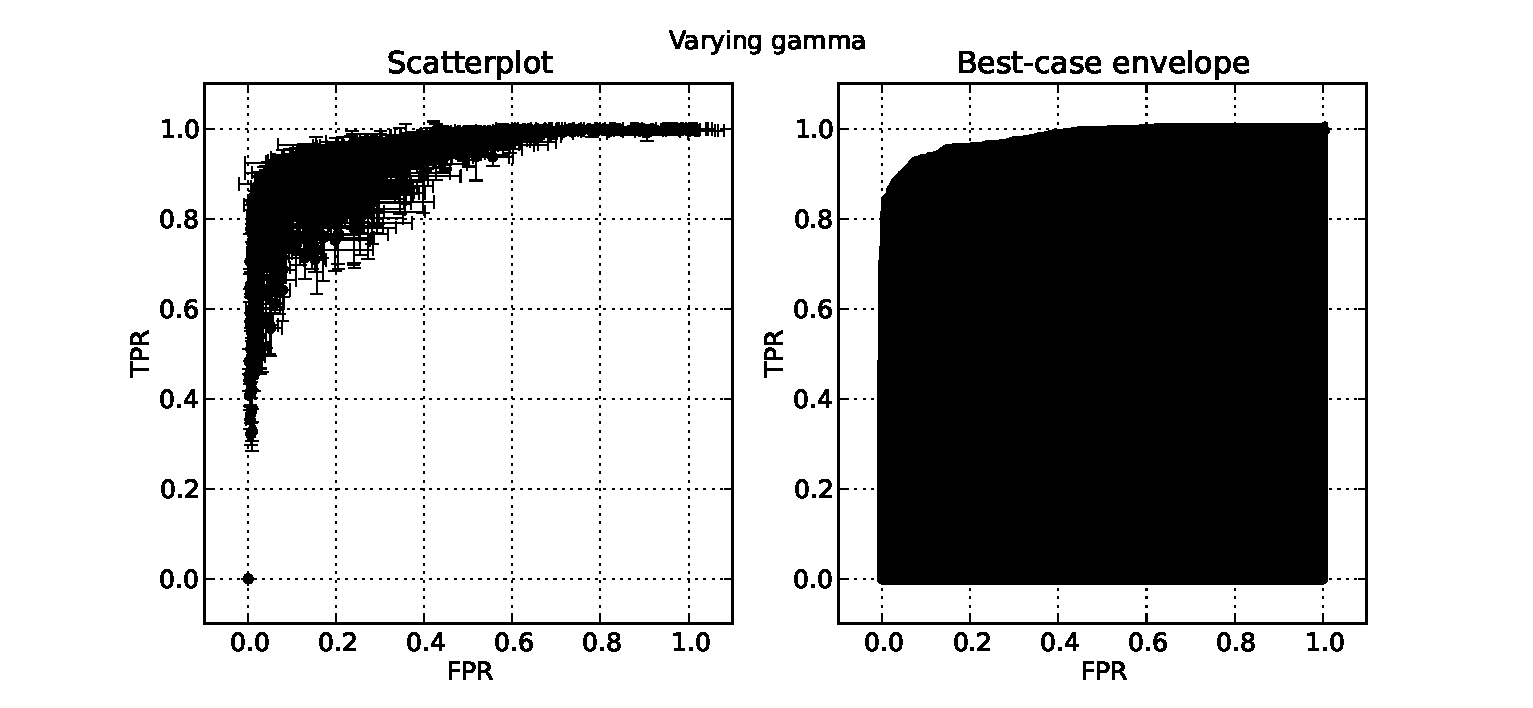
\includegraphics[height=2.5in]{../fig/final/scatter_env/gamma}
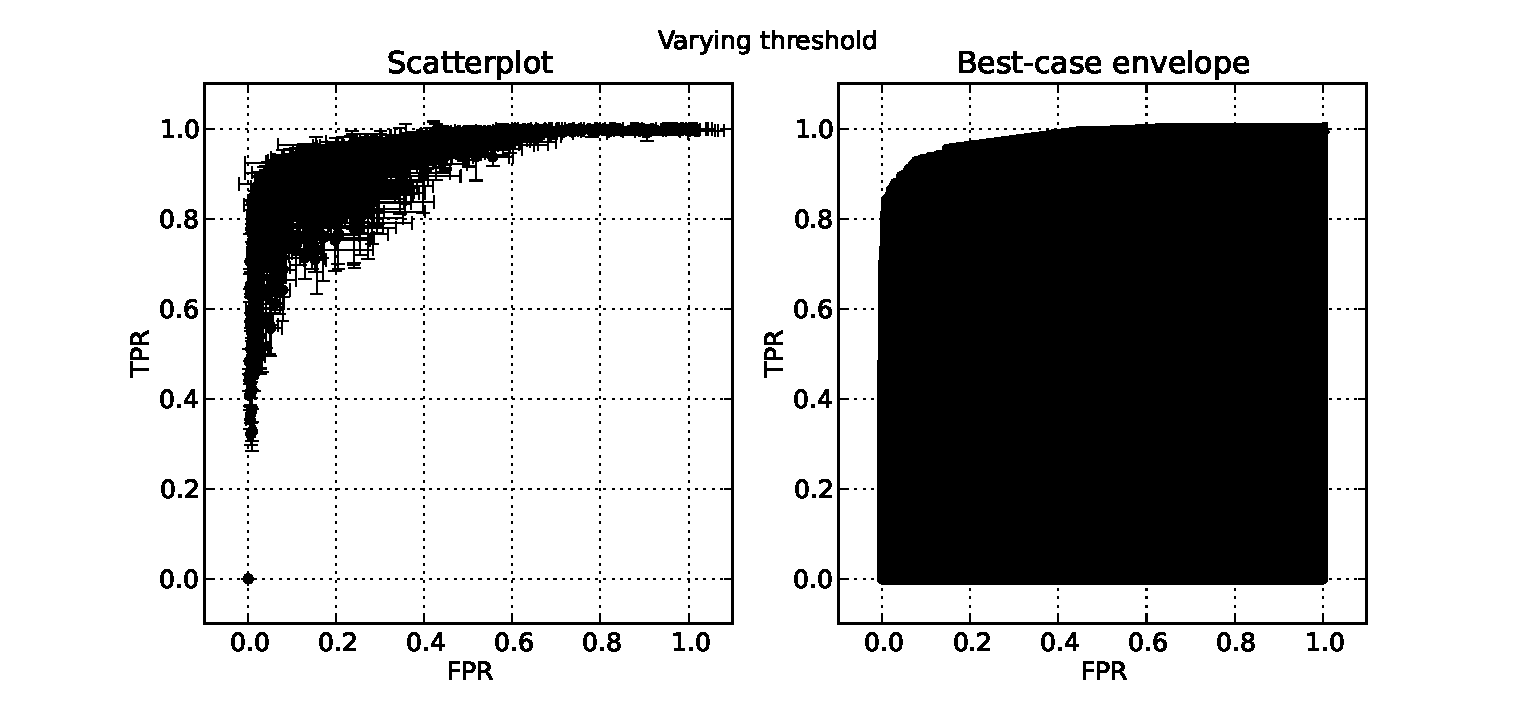
\includegraphics[height=2.5in]{../fig/final/scatter_env/threshold}
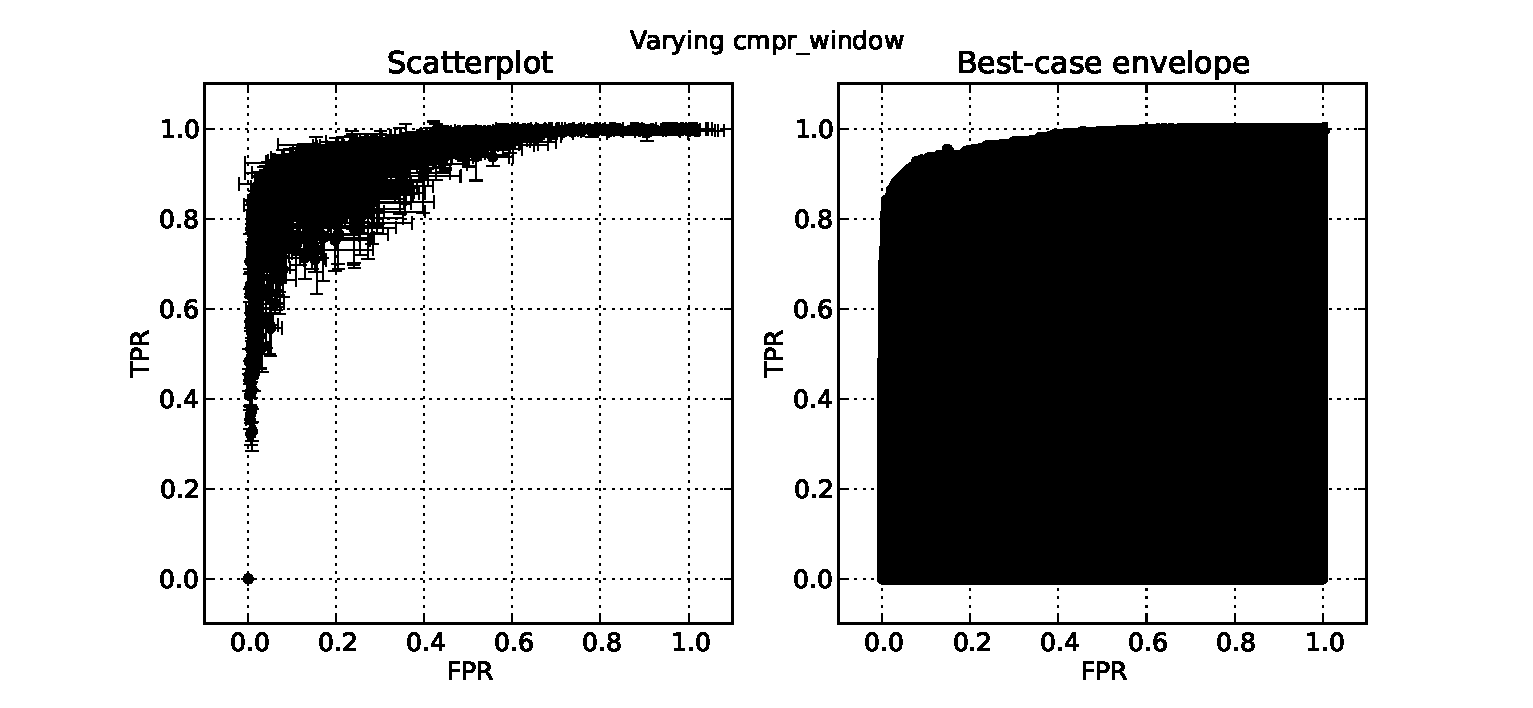
\includegraphics[height=2.5in]{../fig/final/scatter_env/cmpr_window}
\end{center}
\caption{\label{fig:roc_env2}}
\end{figure}

\begin{figure}[!h]
\begin{center}
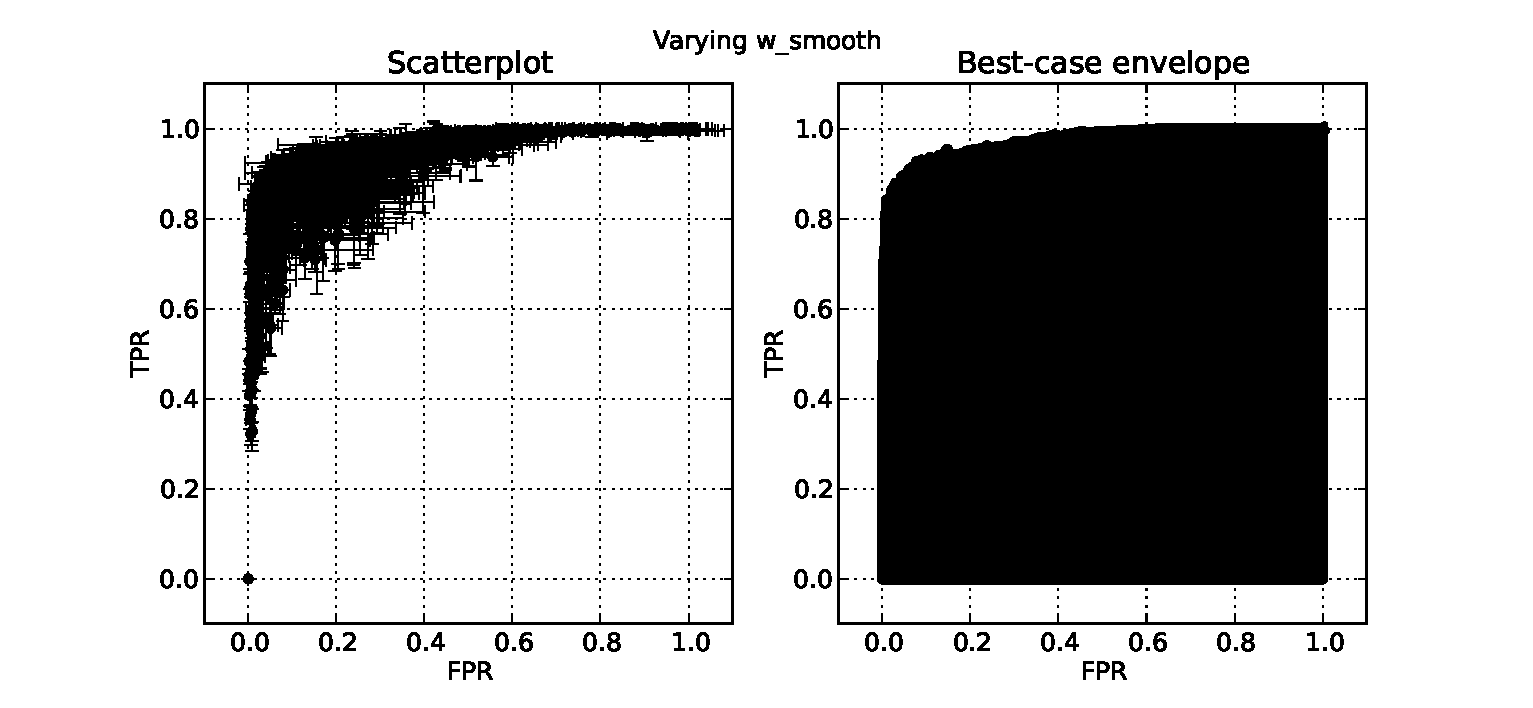
\includegraphics[height=2.5in]{../fig/final/scatter_env/w_smooth}
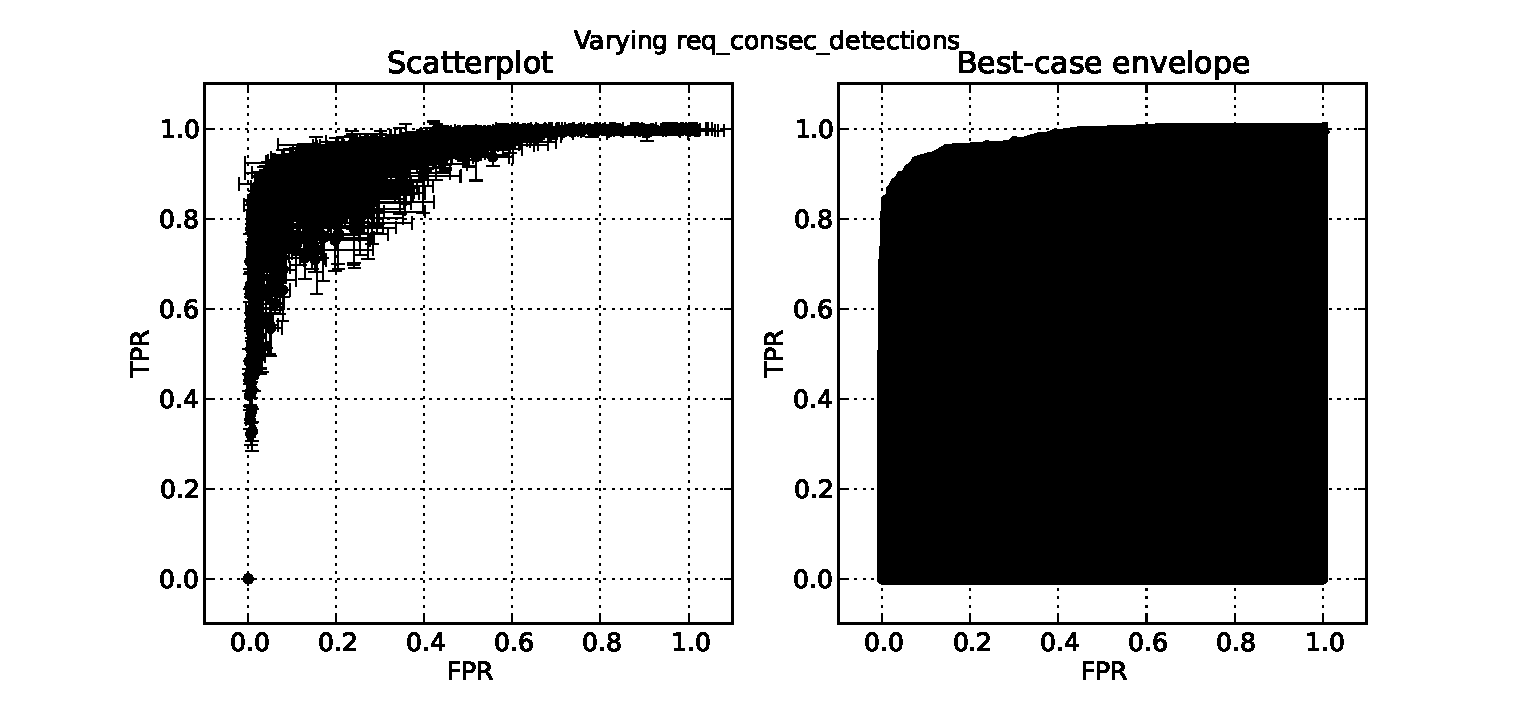
\includegraphics[height=2.5in]{../fig/final/scatter_env/req_consec_detections}
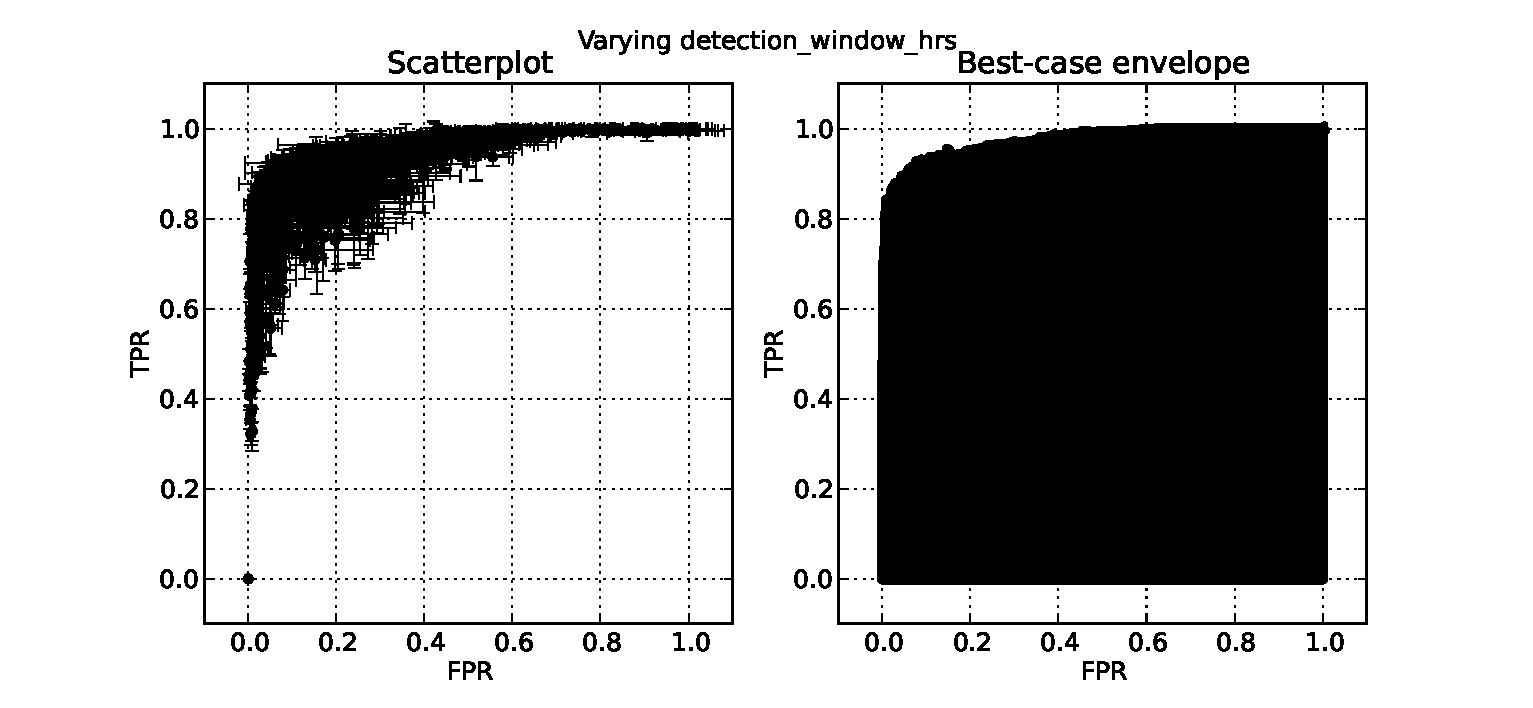
\includegraphics[height=2.5in]{../fig/final/scatter_env/detection_window_hrs}
\end{center}
\caption{\label{fig:roc_env1}}
\end{figure}


\section{Examples} %TODO: Call this something better

True positives. Slow rising vs fast rising.

True negatives.

False positives. Stuff with significant volume or spikes.

False negatives. Stuff with too little volume or not enough spikes.

\section{Effect of Parameters}

Do we move up or down the curve?

We show how varying a given parameter $p$ trades off $FPR$ for $TPR$ by
computing the discrete derivative of $FPR$ and $TPR$ with respect to $p$. For
each ROC curve, corresponding to the variable parameter $p$ and some fixed
combination of remaining parameters, we compute
\begin{gather}
\Delta_{p,i}^{FPR} = \frac{FPR(p_{i}) - FPR(p_{i-1})}{p_i - p_{i-1}}\\
\Delta_{p,i}^{TPR} = \frac{TPR(p_{i}) - TPR(p_{i-1})}{p_i - p_{i-1}}
\end{gather}
for each ROC curve associated with $p$ and for $i$ ranging from the second to the last value
of $p$ in increasing order. If each point on the ROC curve is produced by
multiple trials, we compute the above for all possible combinations of ROC
curves. Finally, we compute the above across all combinations of fixed
parameters.

The result is a distribution of discrete derivatives of $FPR$ and $TPR$ with
respect to a variable parameter of interest $p$ which highlights the effect of
$p$ on tradeoffs between $FPR$ and $TPR$. We can refer this effect as moving
``up'' the ROC curve, or ``down'' the ROC curve. If most of the mass of
$\Delta_{p}^{FPR}$ and $\Delta_{p}^{TPR}$ is at values greater than 0, then an
increase in $p$ causes a decrease in $FPR$ at the expense of lower $TPR$, moving
down the curve. If, on the other hand, most of the mass is at values less than
zero, an increase in $p$ causes an increase in $TPR$ at the expensive of higher
$FPR$, moving up the curve.

Figure \ref{fig:deltas} shows this effect for each parameter.

\begin{figure}[!h]
\begin{center}
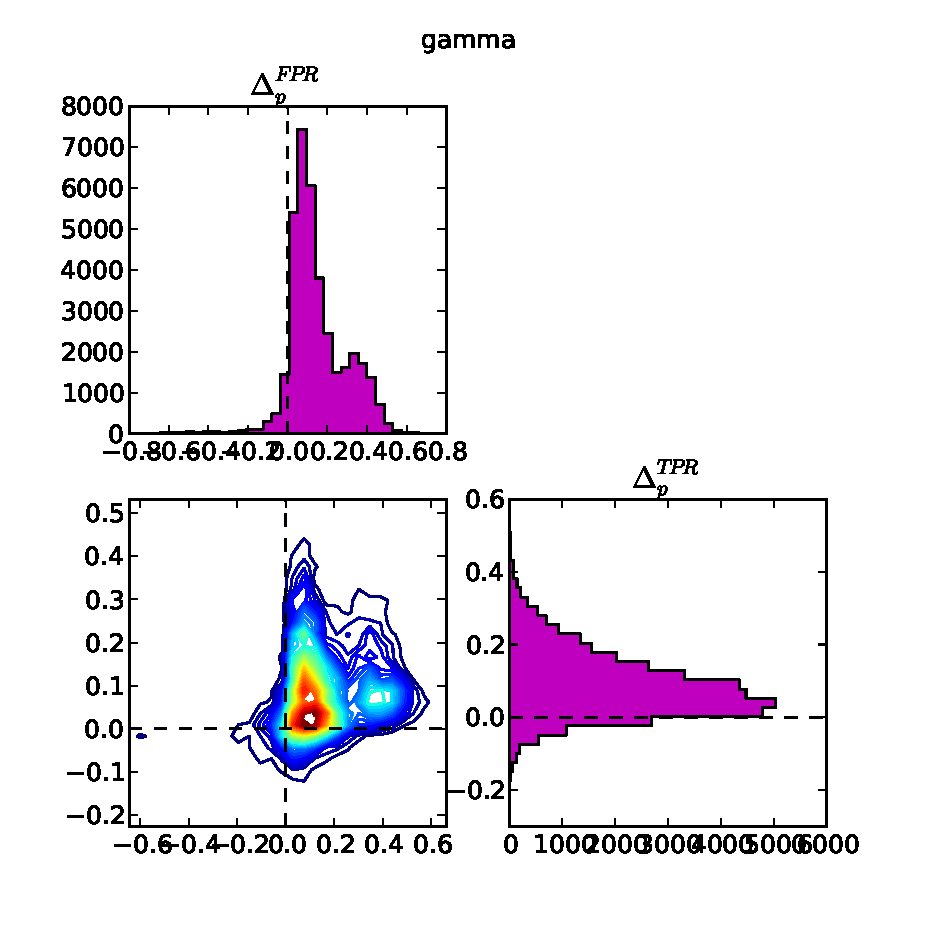
\includegraphics[width=4in]{../fig/final/delta_hist/gamma}
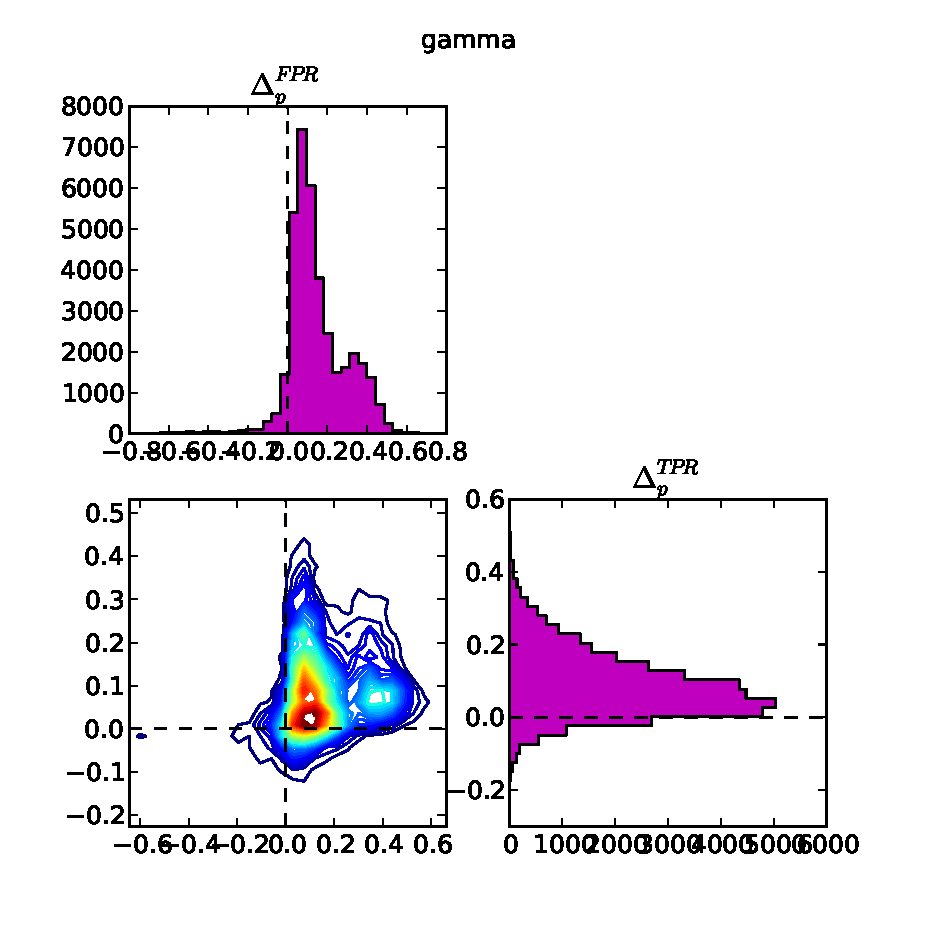
\includegraphics[width=4in]{../fig/final/delta_hist/gamma}
\end{center}
\caption{\label{fig:deltas1}}
\end{figure}

\begin{figure}[!h]
\begin{center}
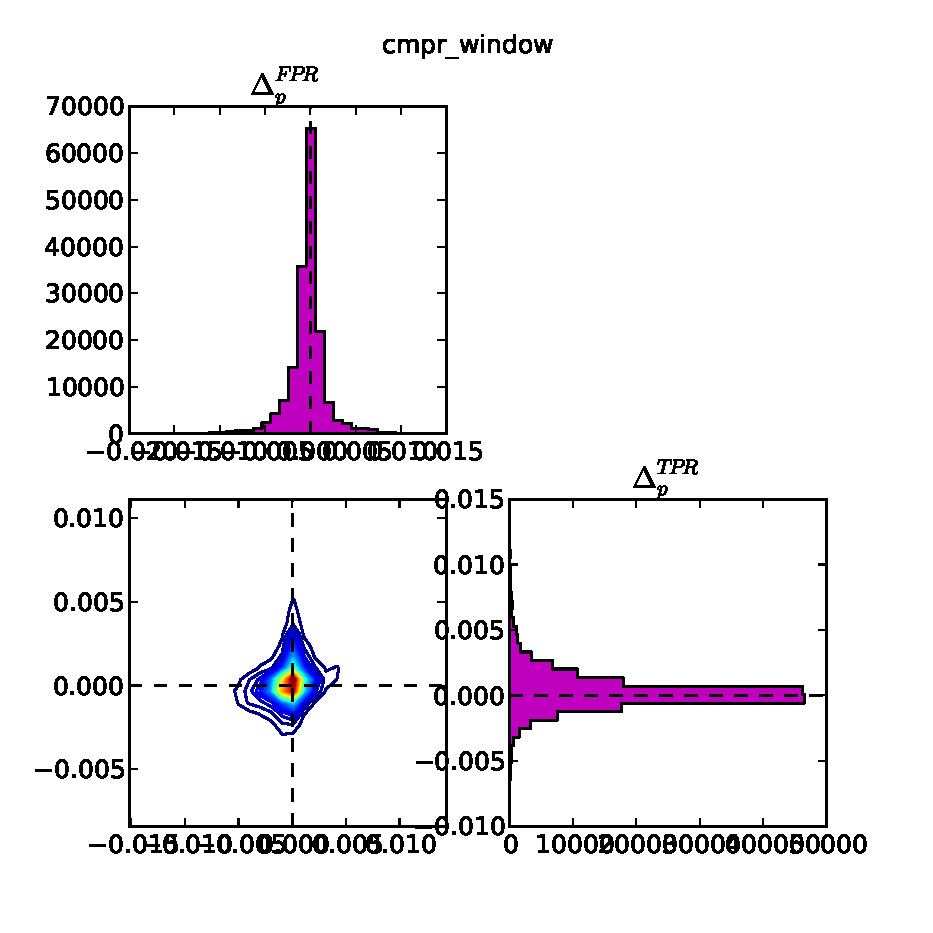
\includegraphics[width=4in]{../fig/final/delta_hist/cmpr_window}
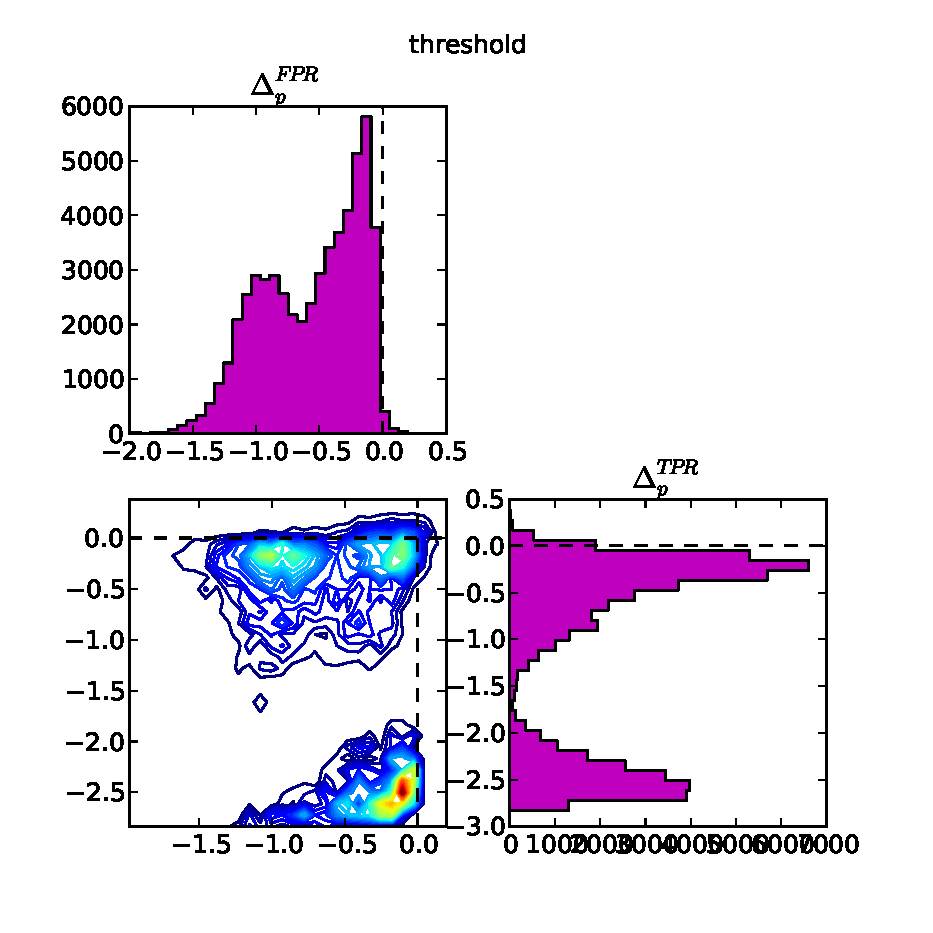
\includegraphics[width=4in]{../fig/final/delta_hist/threshold}
\end{center}
\caption{\label{fig:deltas2}}
\end{figure}

\begin{figure}[!h]
\begin{center}
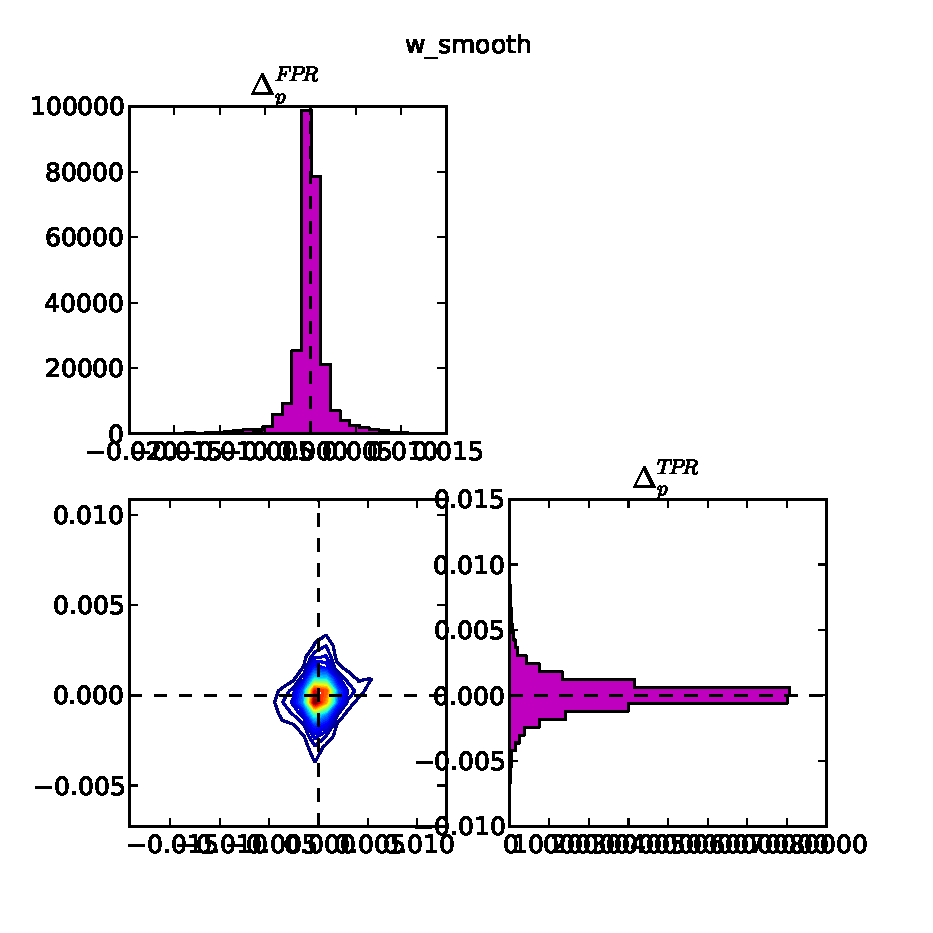
\includegraphics[width=4in]{../fig/final/delta_hist/w_smooth}
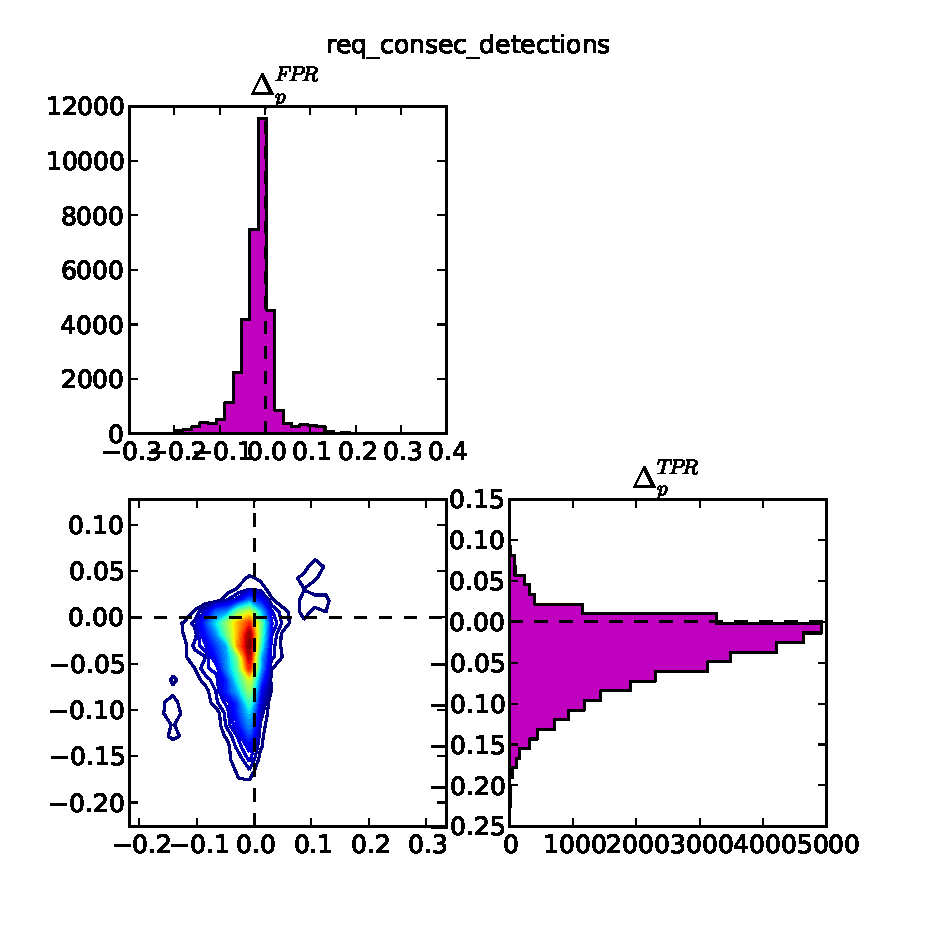
\includegraphics[width=4in]{../fig/final/delta_hist/req_consec_detections}
\end{center}
\caption{\label{fig:deltas3}}
\end{figure}

% TODO: Figure

% TODO: consistent effect, vs contingent effect
It is clear that varying some parameters has the same effect regardless of the
remaining parameters, at least within the range of values explored. 


%TODO: Delta histograms

Increasing \vt{Gamma} always moves us up the curve.
Increasing \vt{Threshold} always moves us down the curve.
Increasing \vt{ReqConsecDetections} always moves us down the curve.

\clearpage
\begin{figure}[!h]
\begin{center}
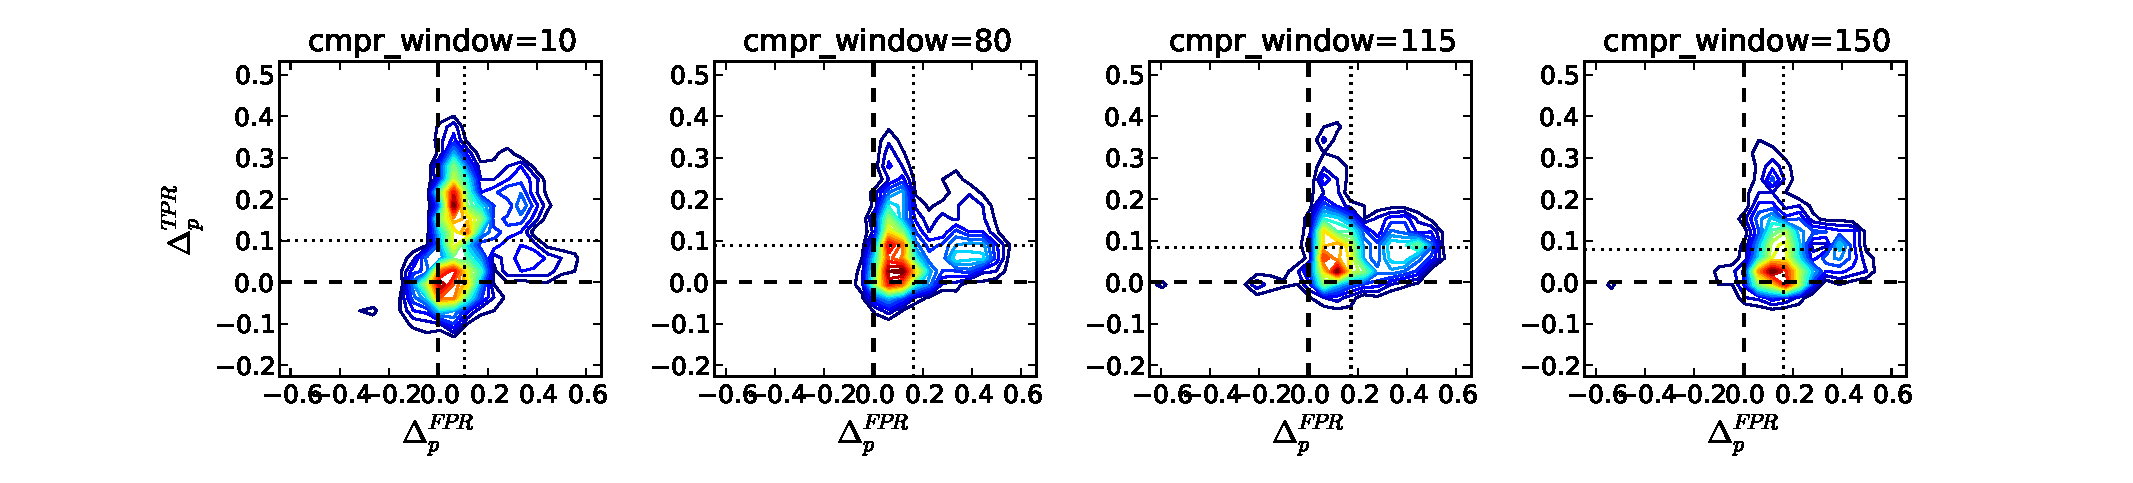
\includegraphics[height=1.5in]{../fig/final/delta_hist_sec/gamma/cmpr_window}
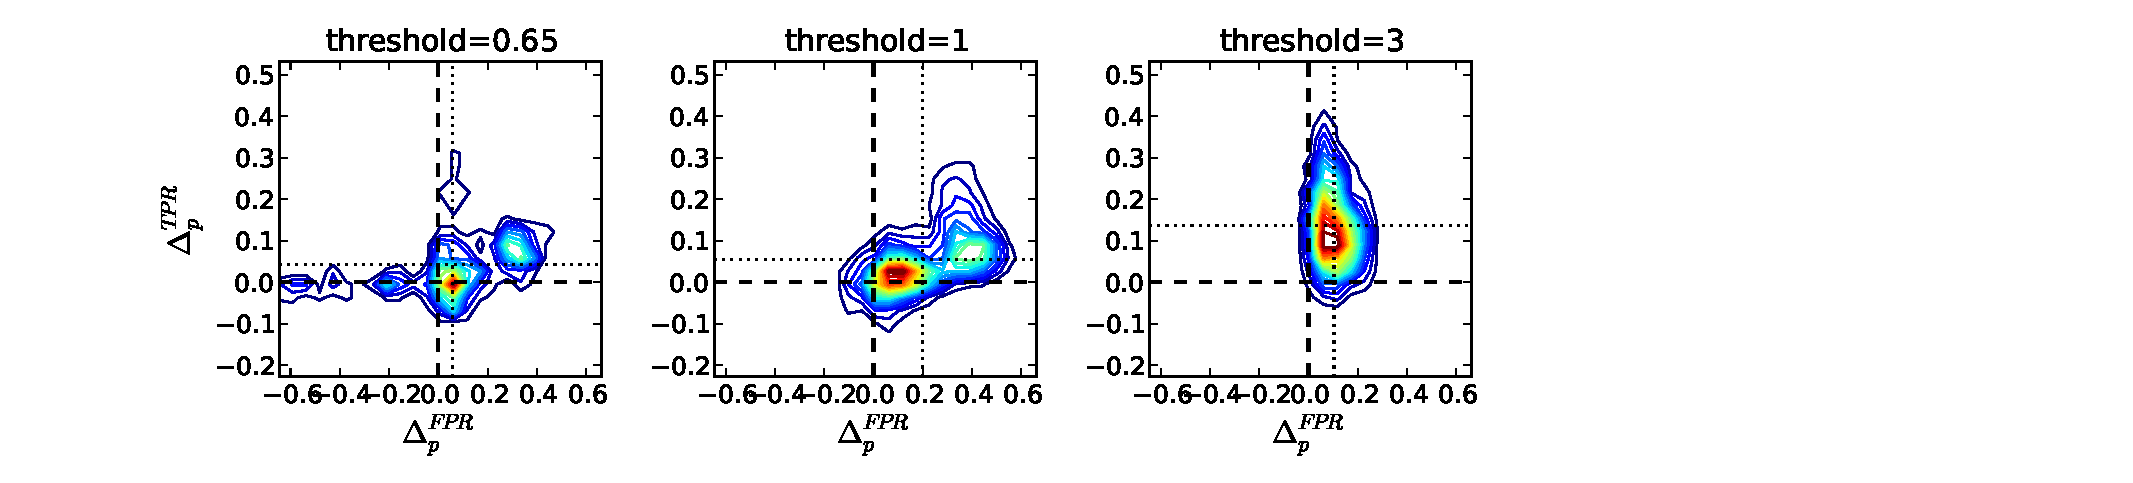
\includegraphics[height=1.5in]{../fig/final/delta_hist_sec/gamma/threshold}
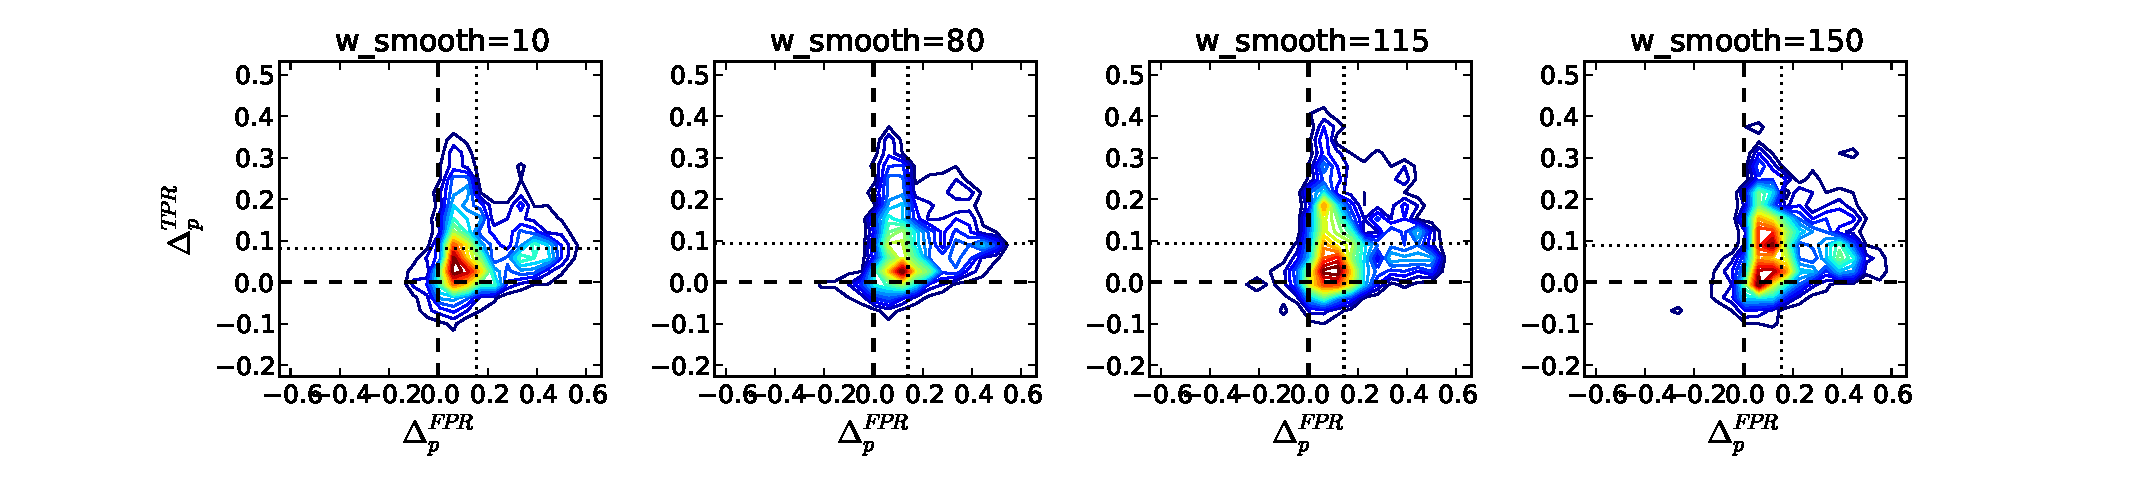
\includegraphics[height=1.5in]{../fig/final/delta_hist_sec/gamma/w_smooth}
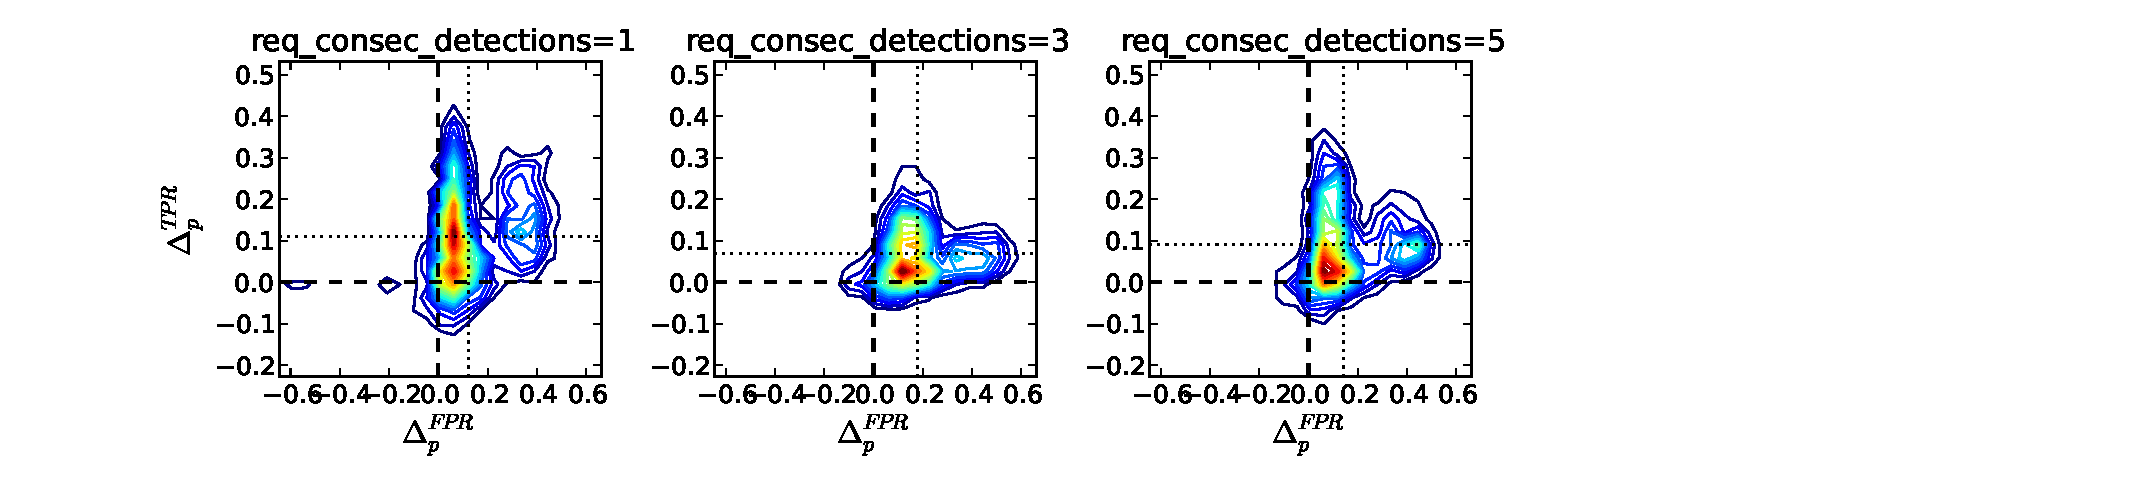
\includegraphics[height=1.5in]{../fig/final/delta_hist_sec/gamma/req_consec_detections}
\end{center}
\caption{\label{fig:delta_sec1} Secondary effects of parameters for a varying \vt{Gamma}}
\end{figure}

\begin{figure}[!h]
\begin{center}
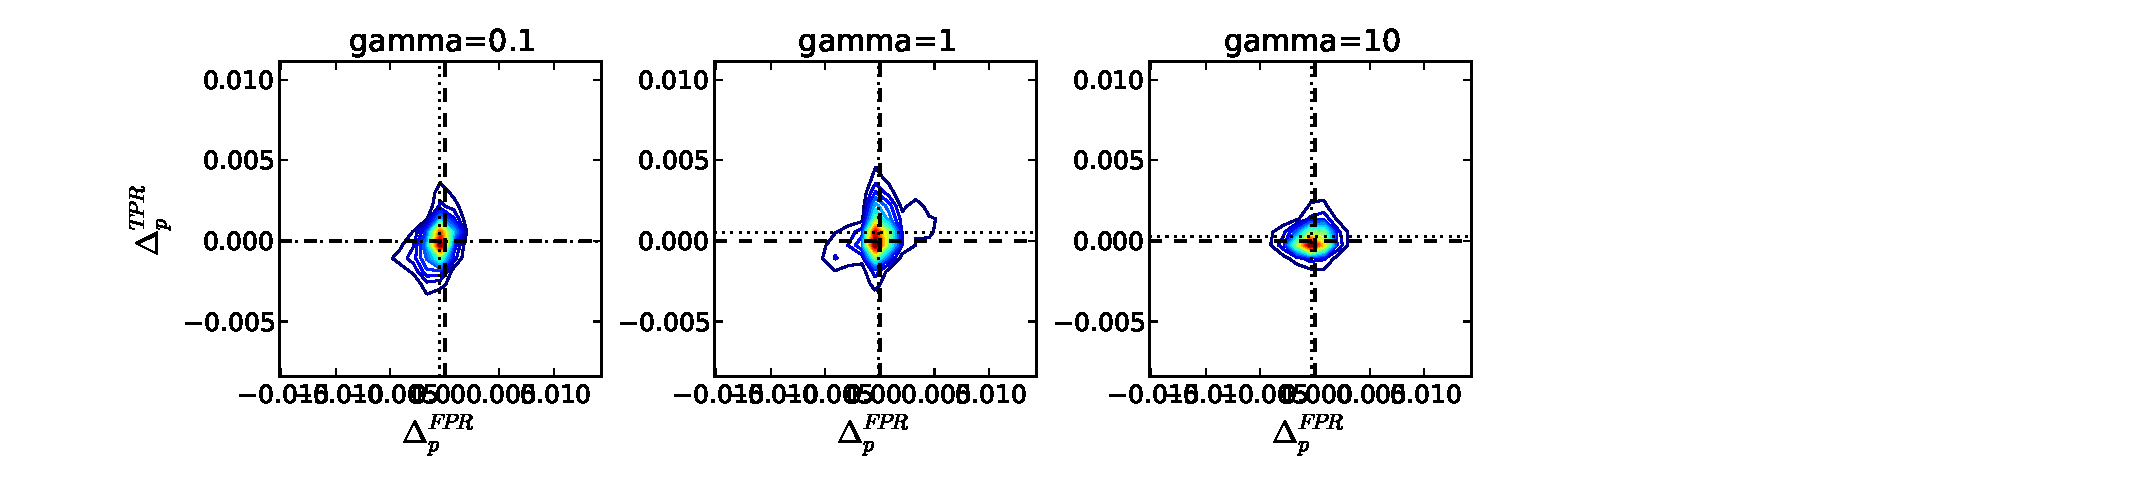
\includegraphics[height=1.5in]{../fig/final/delta_hist_sec/cmpr_window/gamma}
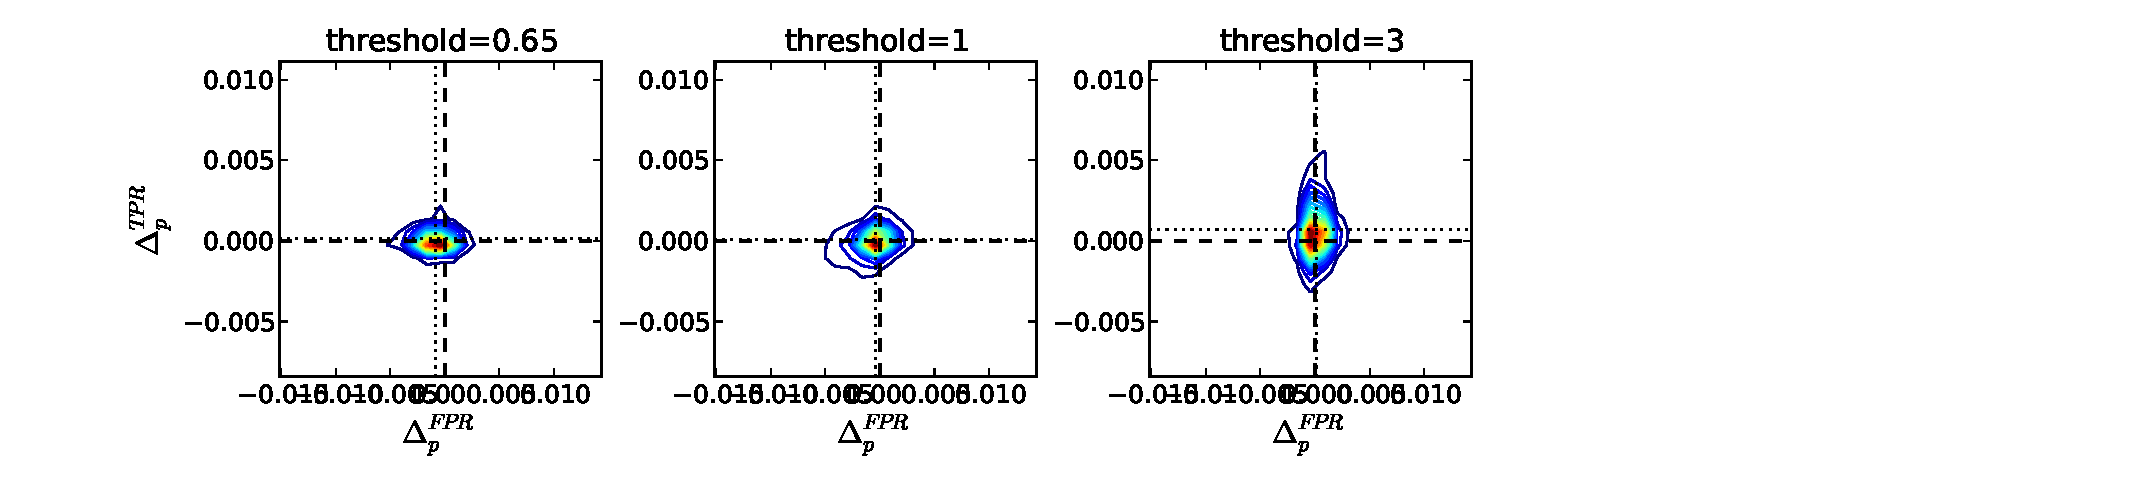
\includegraphics[height=1.5in]{../fig/final/delta_hist_sec/cmpr_window/threshold}
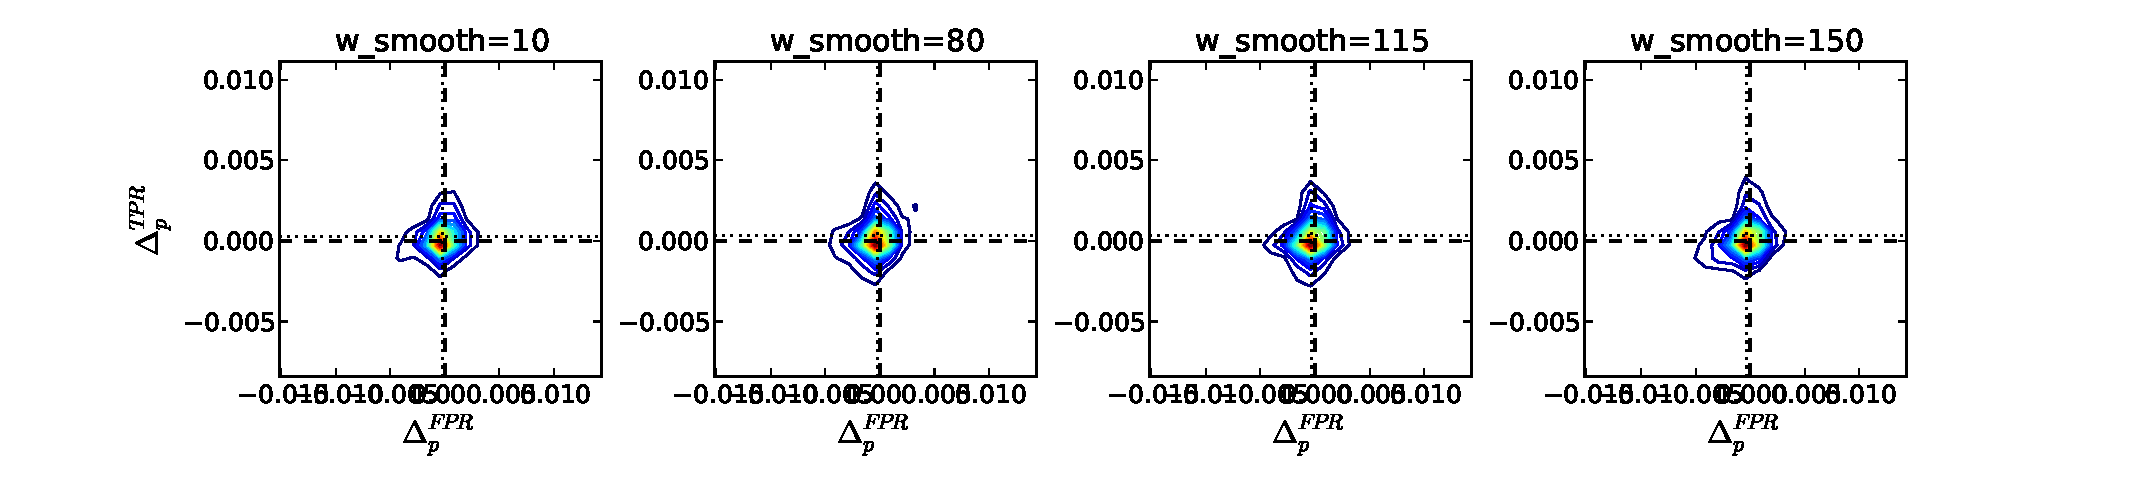
\includegraphics[height=1.5in]{../fig/final/delta_hist_sec/cmpr_window/w_smooth}
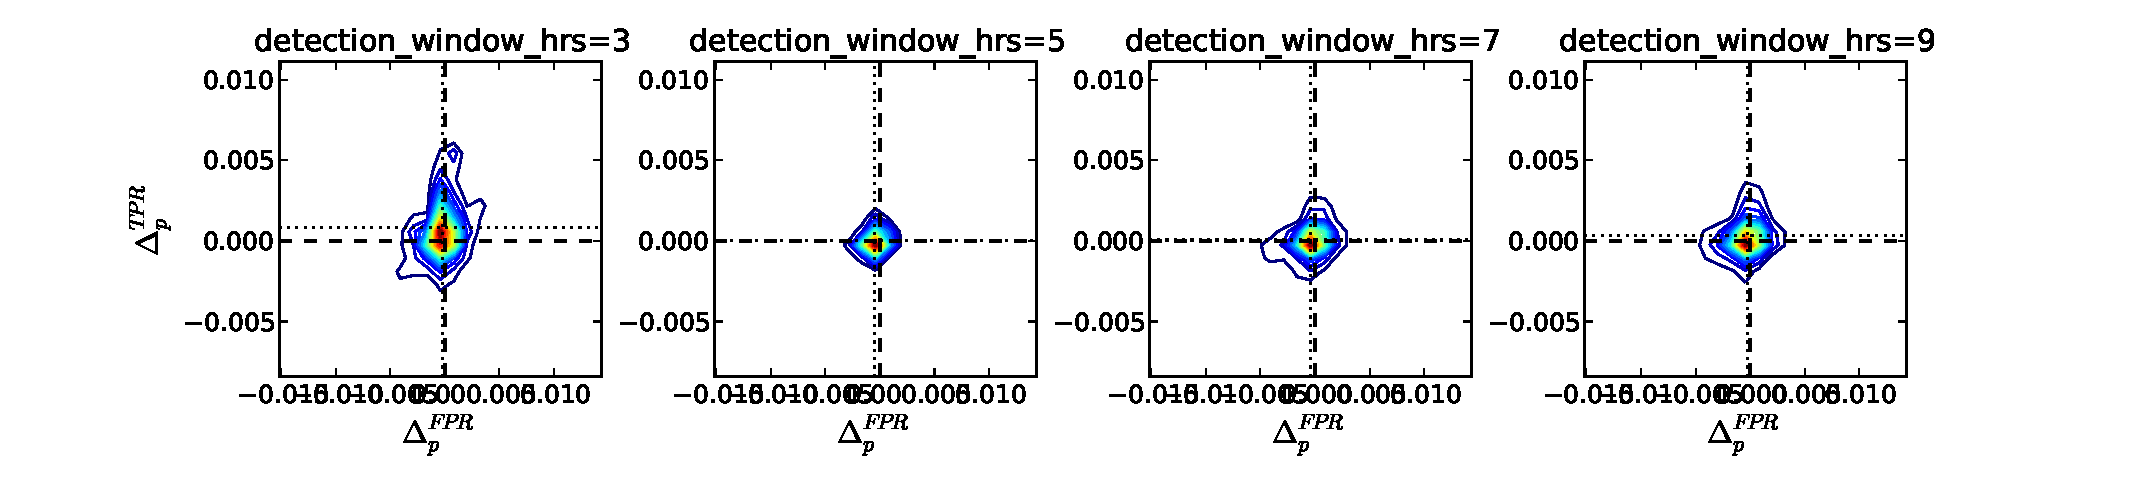
\includegraphics[height=1.5in]{../fig/final/delta_hist_sec/cmpr_window/detection_window_hrs}
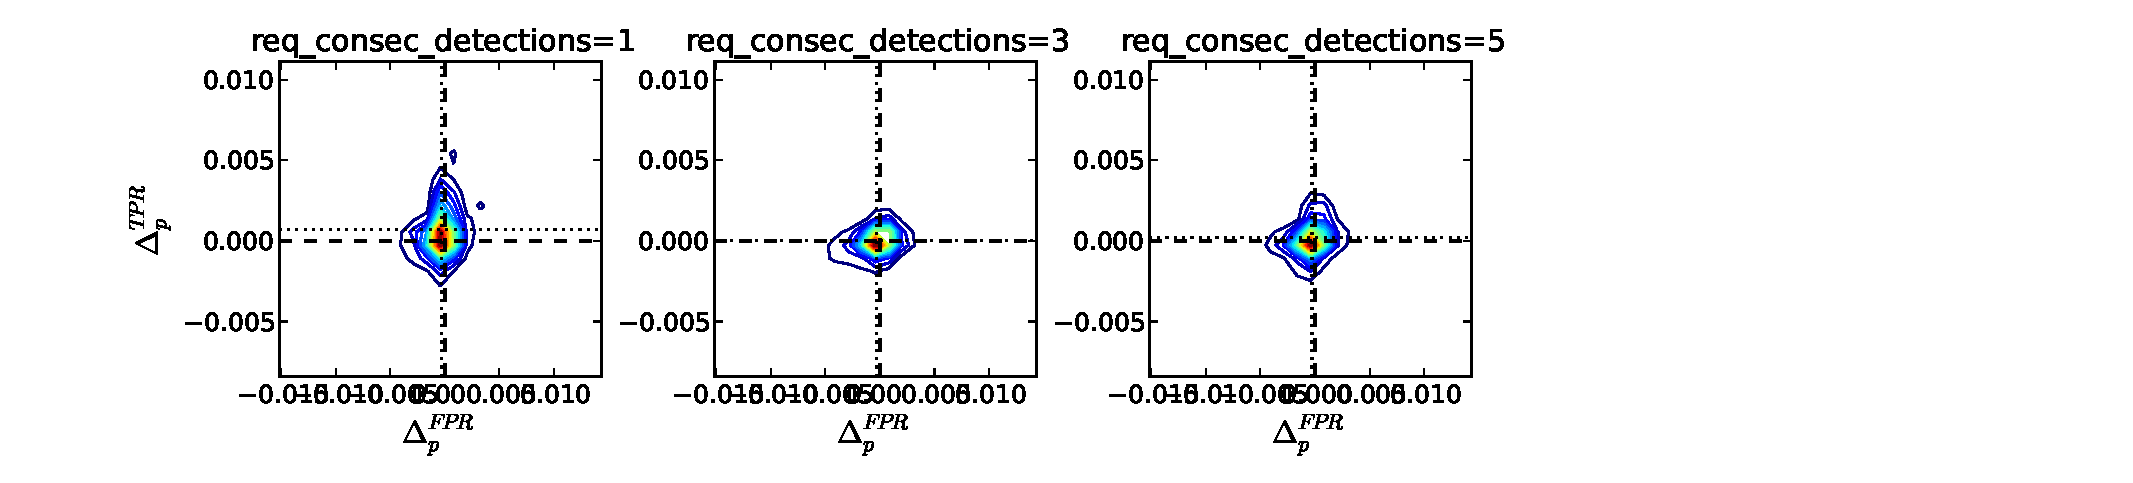
\includegraphics[height=1.5in]{../fig/final/delta_hist_sec/cmpr_window/req_consec_detections}
\end{center}
\caption{\label{fig:delta_sec2} Secondary effects of parameters for a varying \vt{CmprWindow}}
\end{figure}

\begin{figure}[!h]
\begin{center}
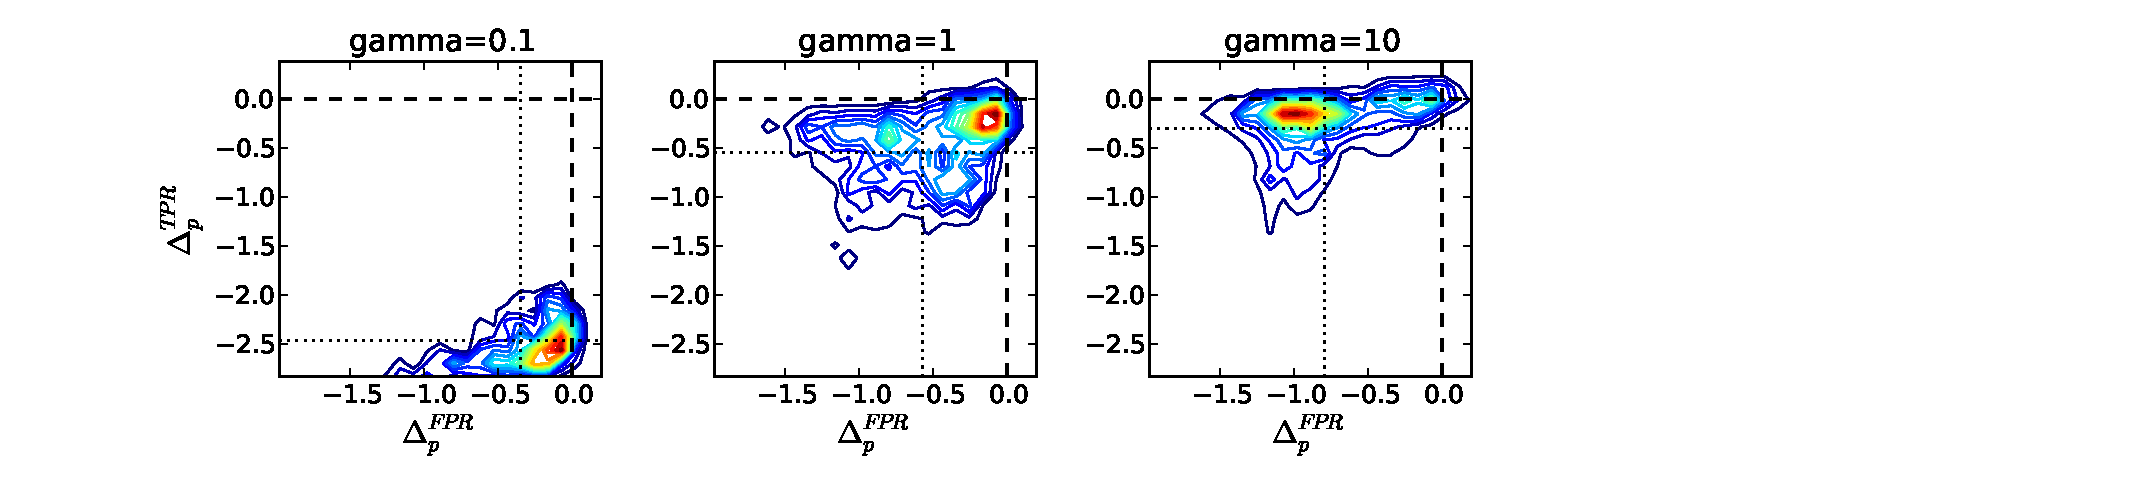
\includegraphics[height=1.5in]{../fig/final/delta_hist_sec/threshold/gamma}
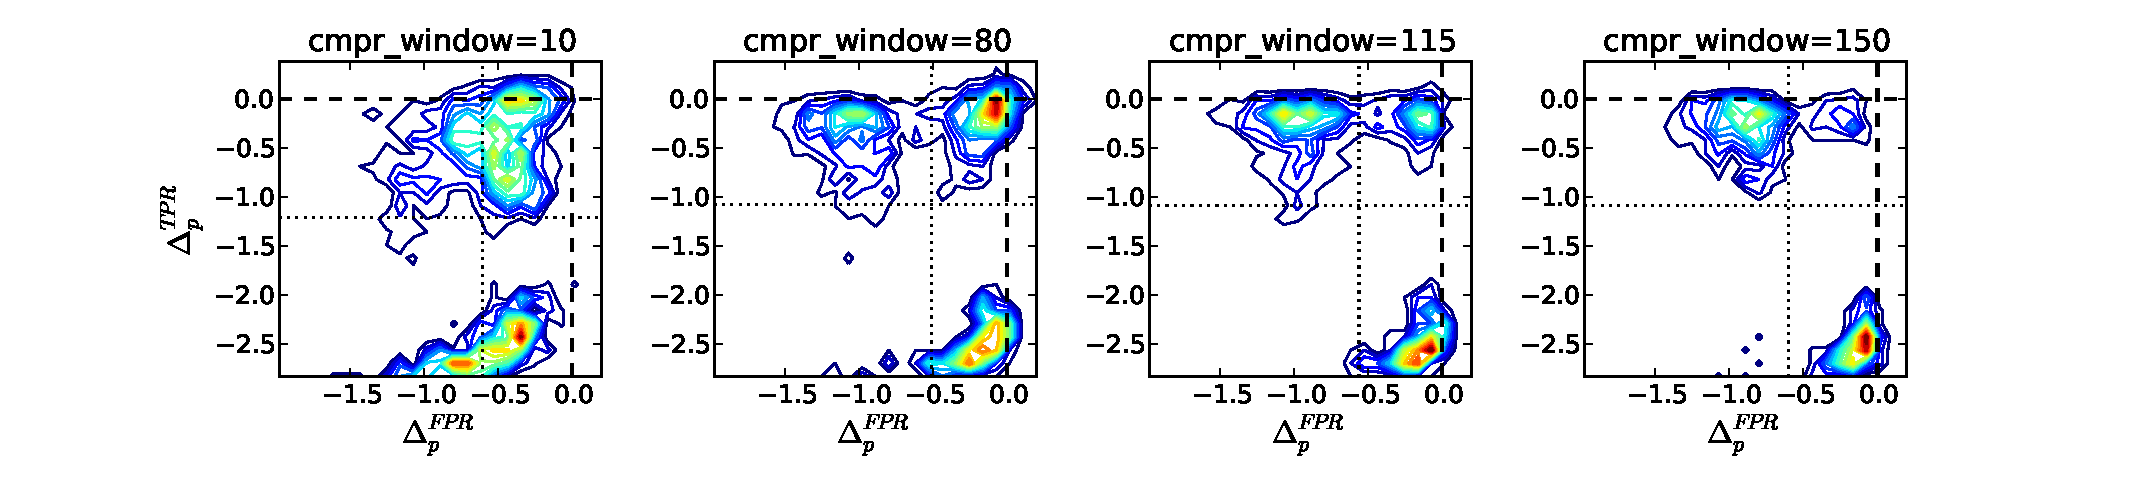
\includegraphics[height=1.5in]{../fig/final/delta_hist_sec/threshold/cmpr_window}
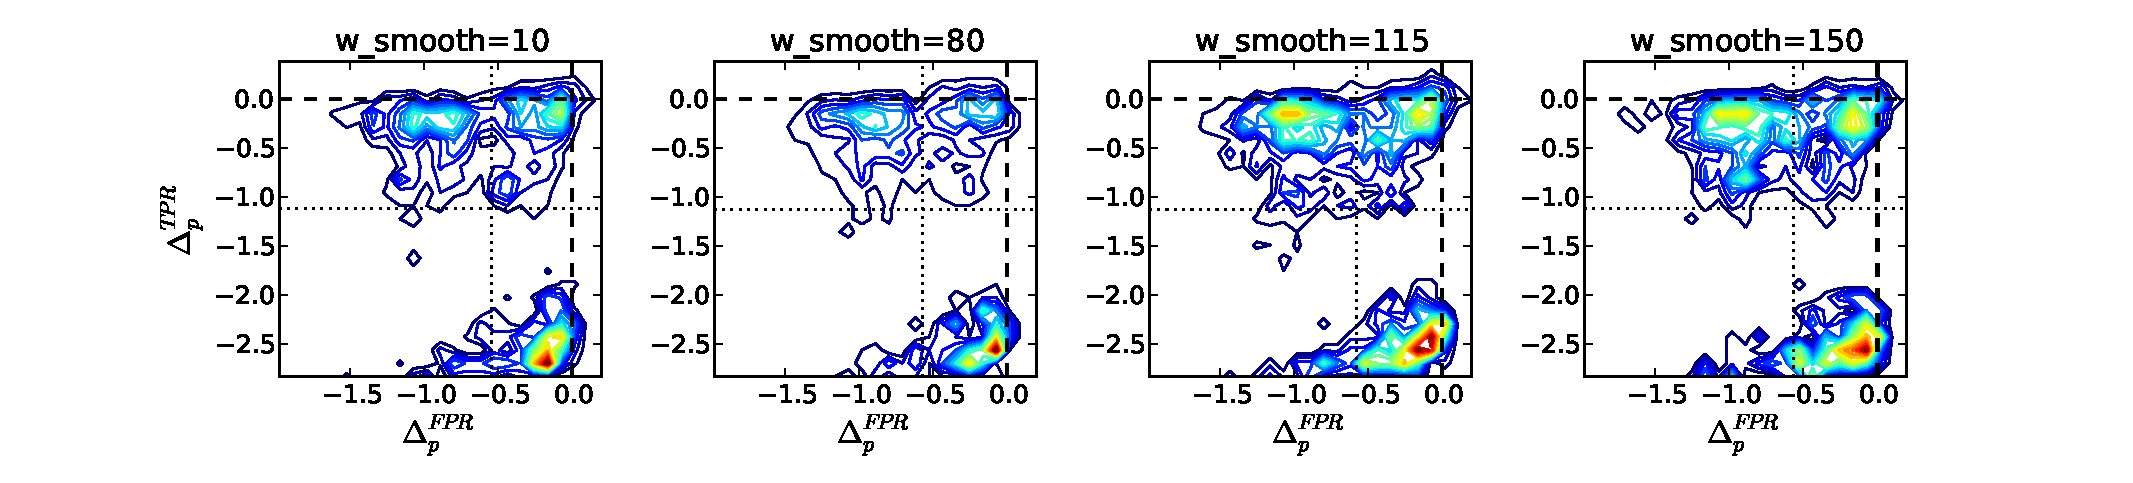
\includegraphics[height=1.5in]{../fig/final/delta_hist_sec/threshold/w_smooth}
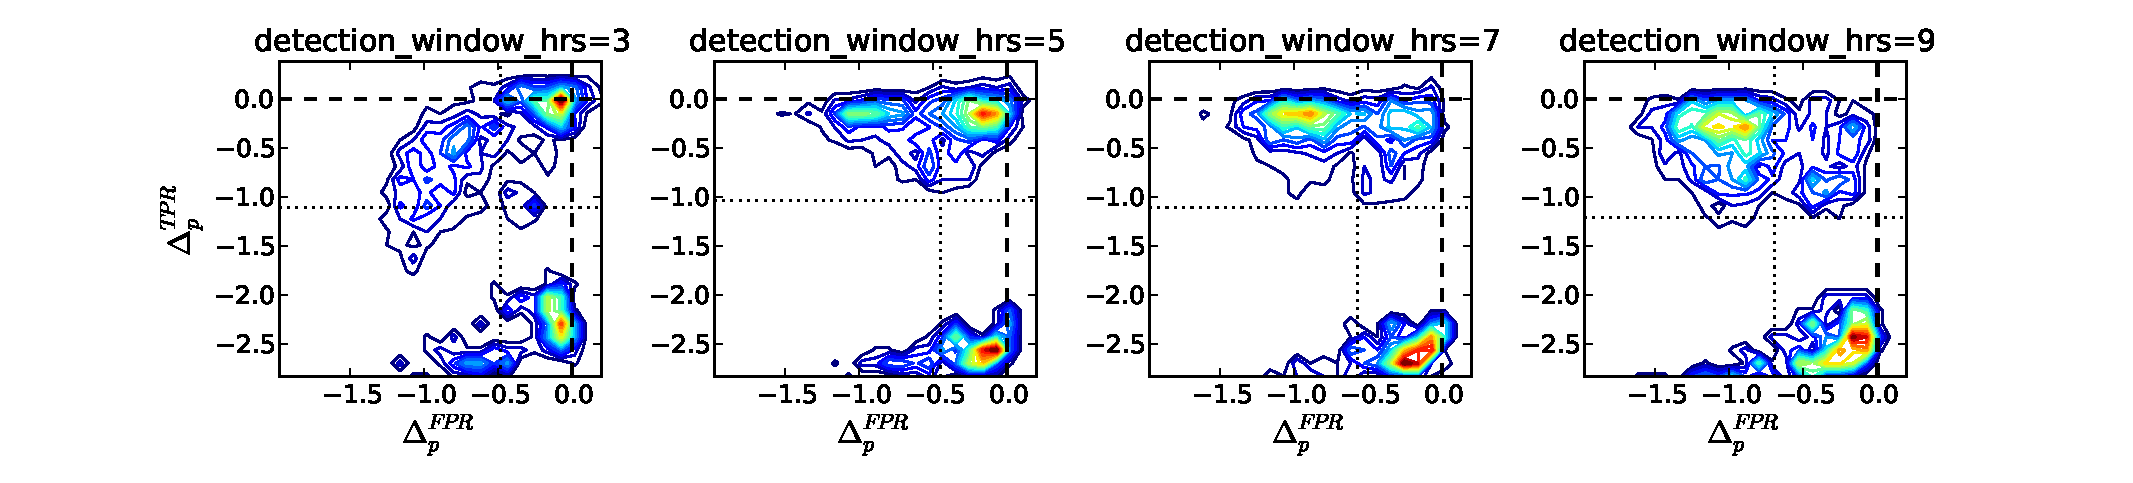
\includegraphics[height=1.5in]{../fig/final/delta_hist_sec/threshold/detection_window_hrs}
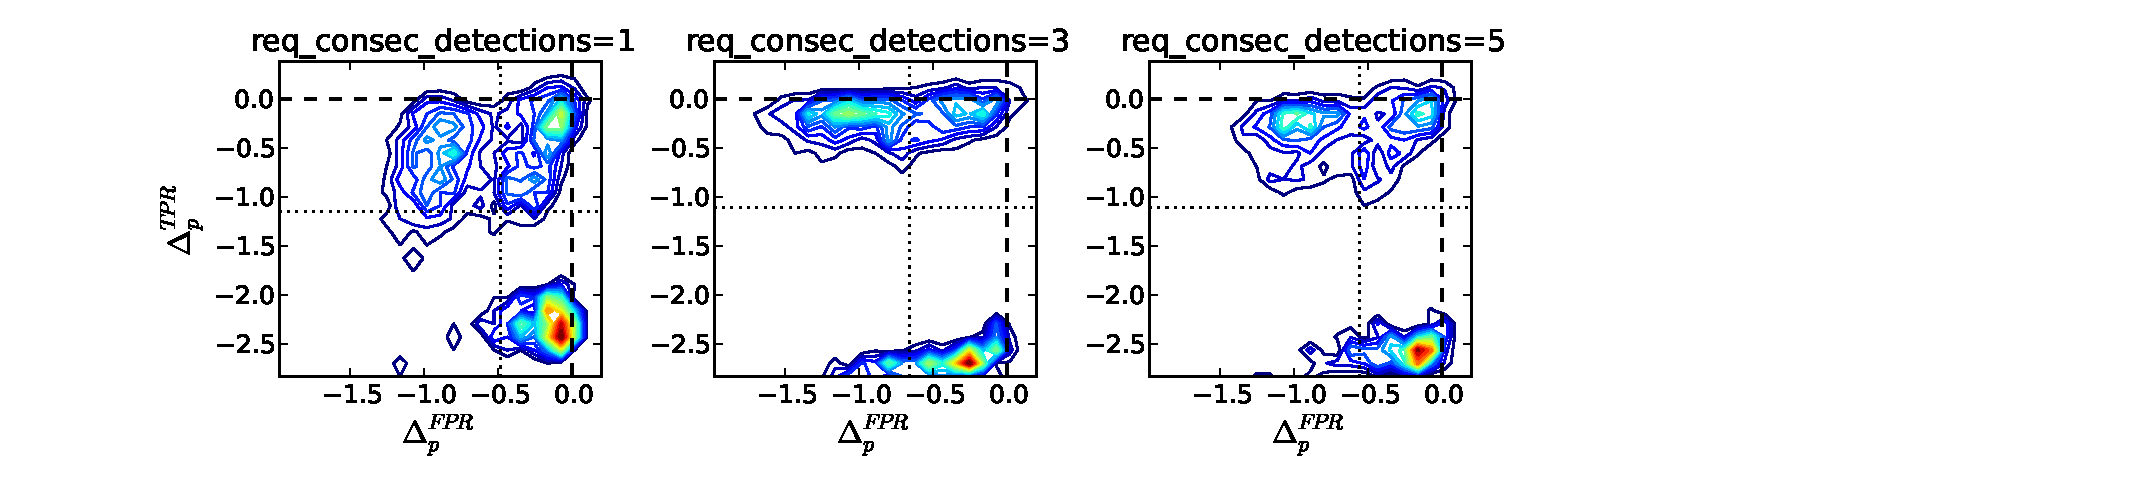
\includegraphics[height=1.5in]{../fig/final/delta_hist_sec/threshold/req_consec_detections}
\end{center}
\caption{\label{fig:delta_sec3} Secondary effects of parameters for a varying \vt{Threshold}}
\end{figure}

\begin{figure}[!h]
\begin{center}
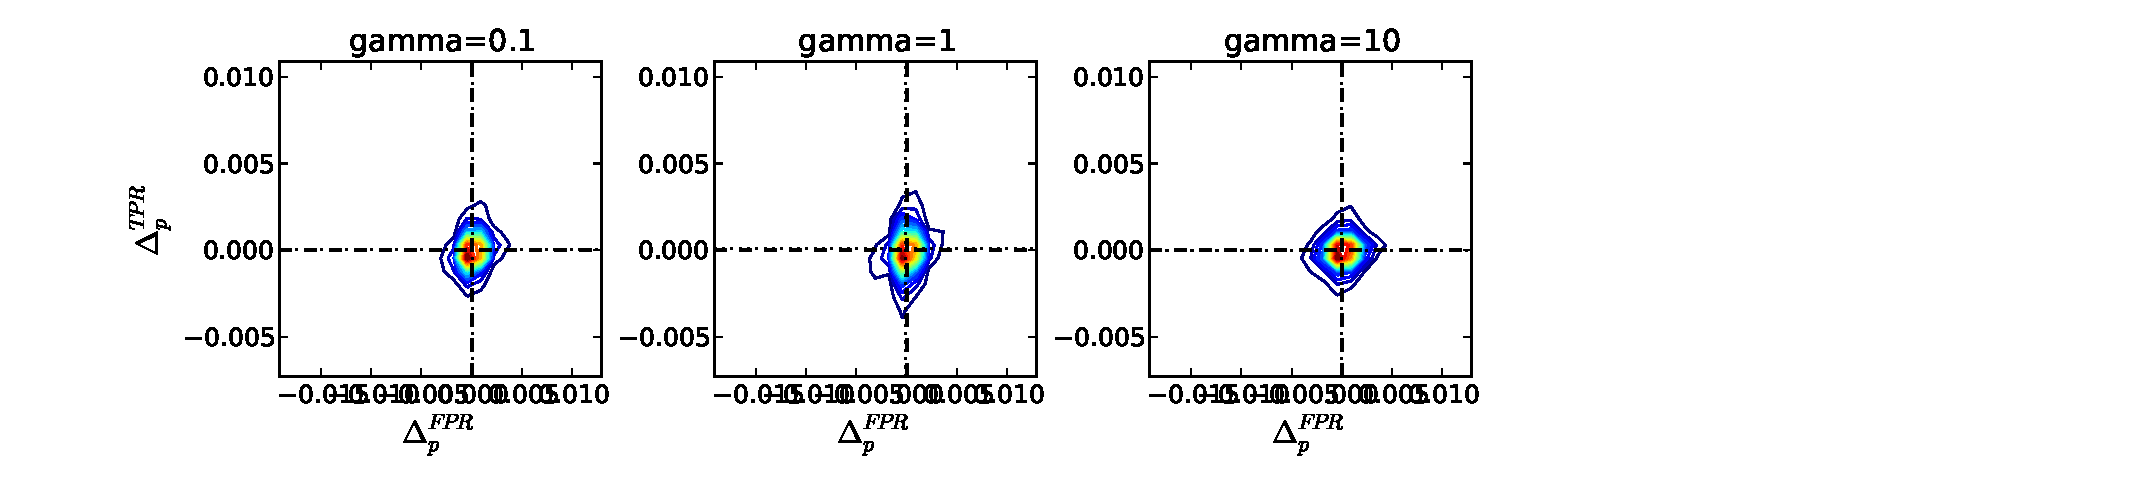
\includegraphics[height=1.5in]{../fig/final/delta_hist_sec/w_smooth/gamma}
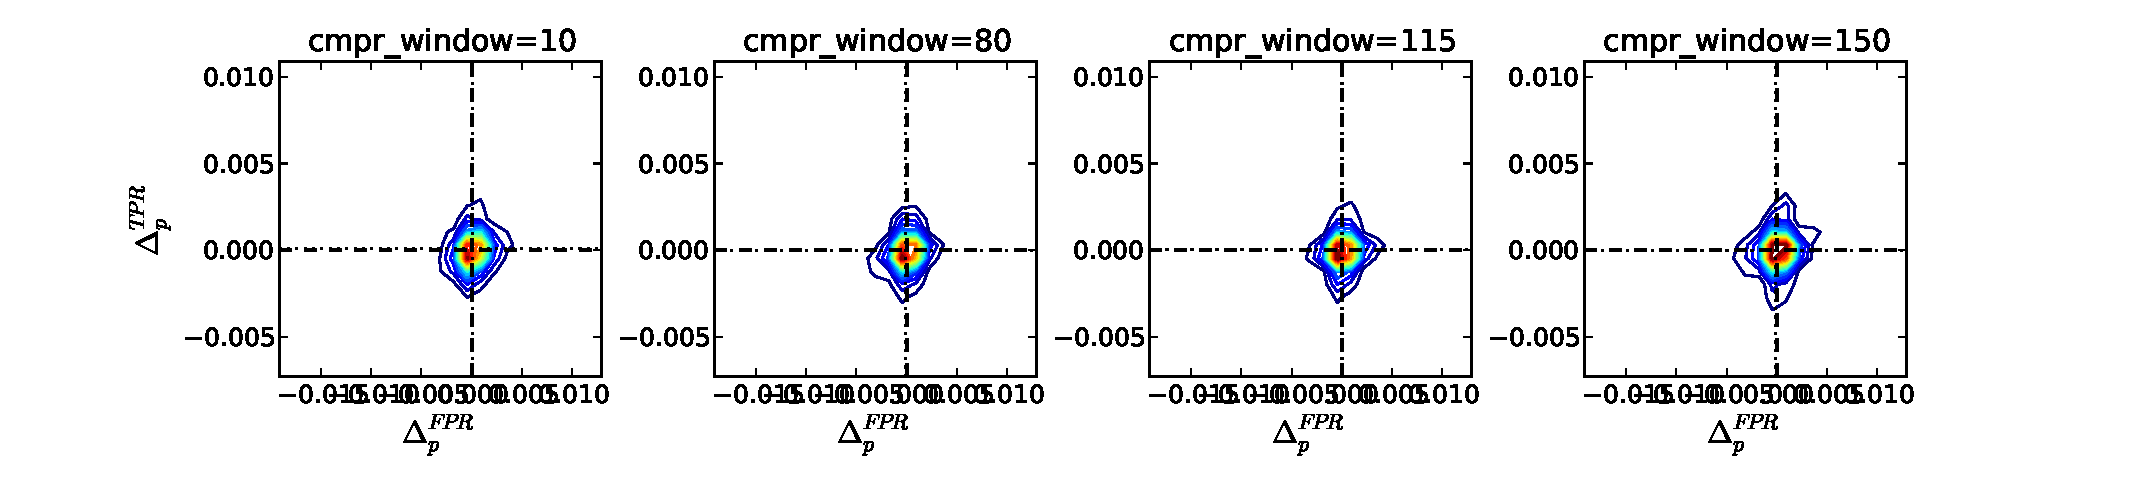
\includegraphics[height=1.5in]{../fig/final/delta_hist_sec/w_smooth/cmpr_window}
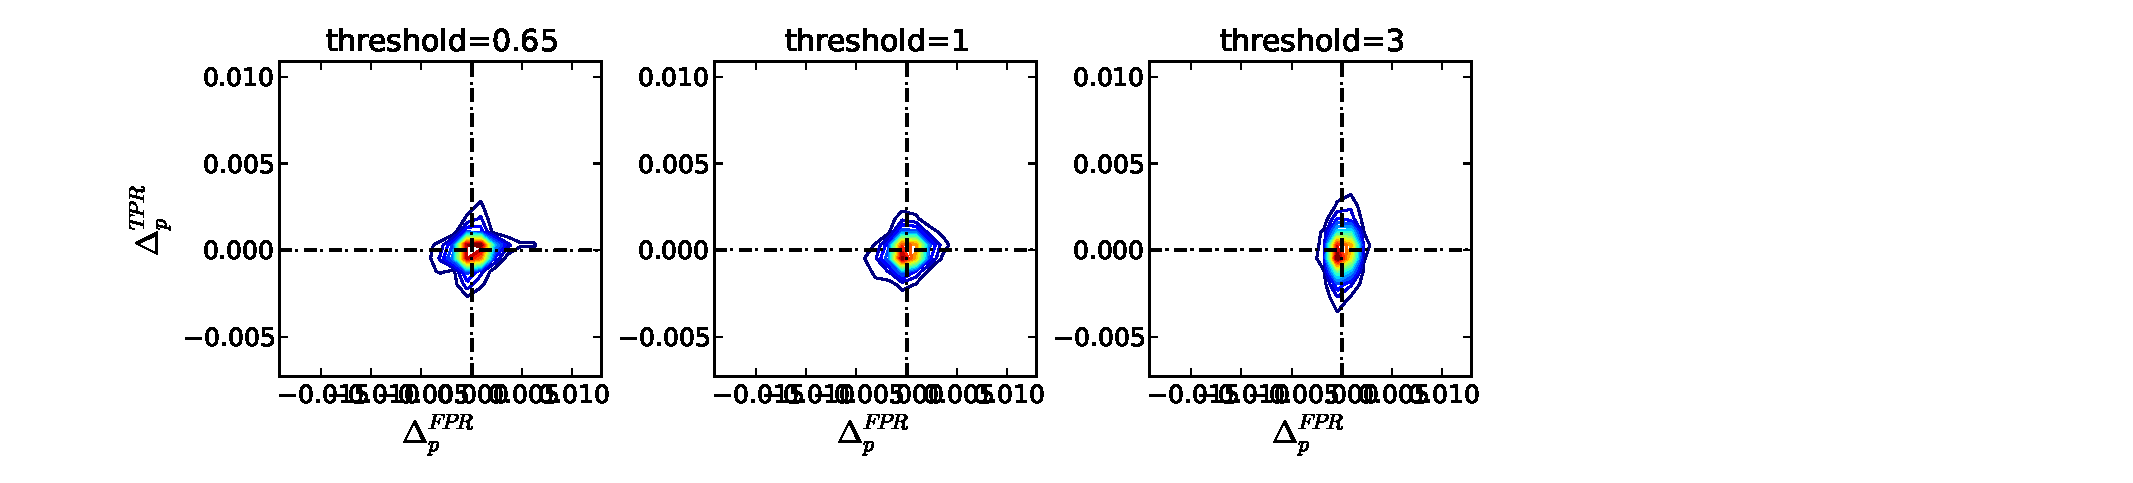
\includegraphics[height=1.5in]{../fig/final/delta_hist_sec/w_smooth/threshold}
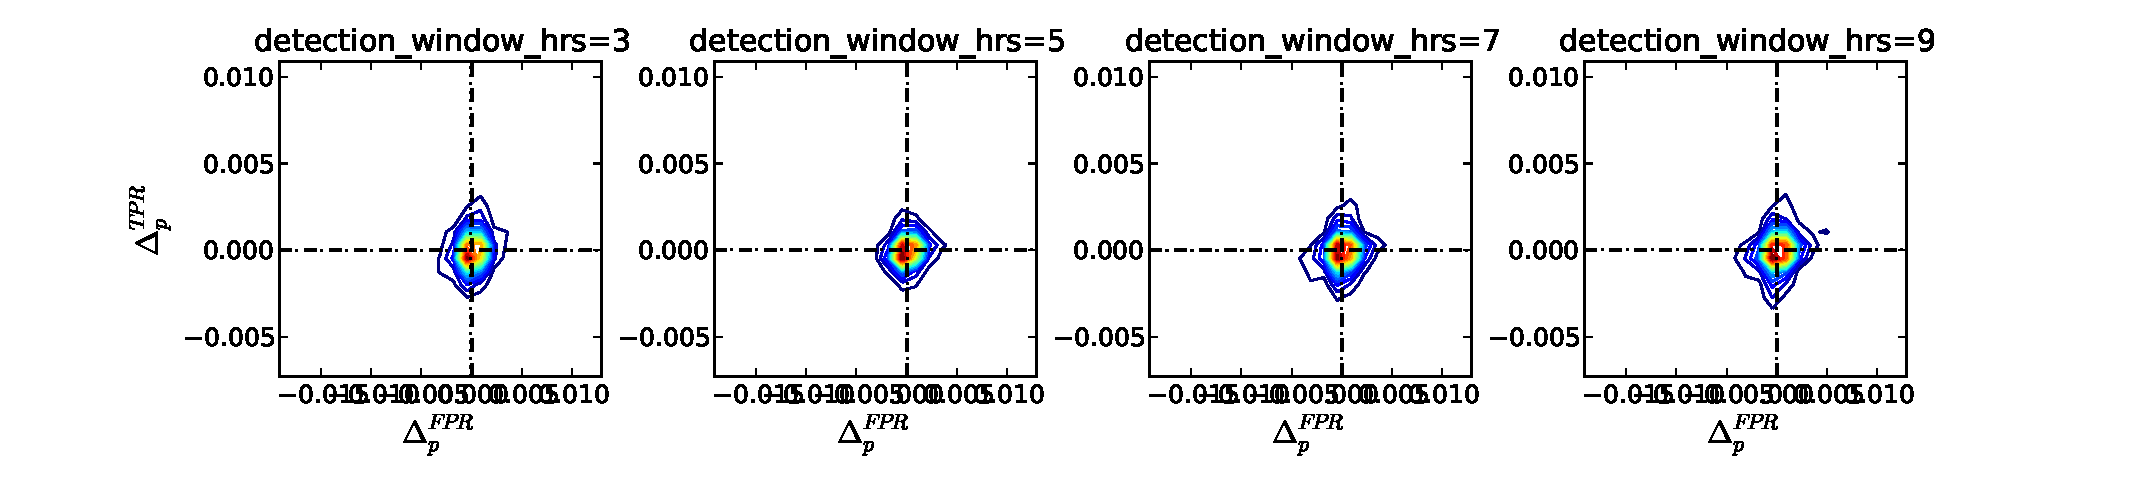
\includegraphics[height=1.5in]{../fig/final/delta_hist_sec/w_smooth/detection_window_hrs}
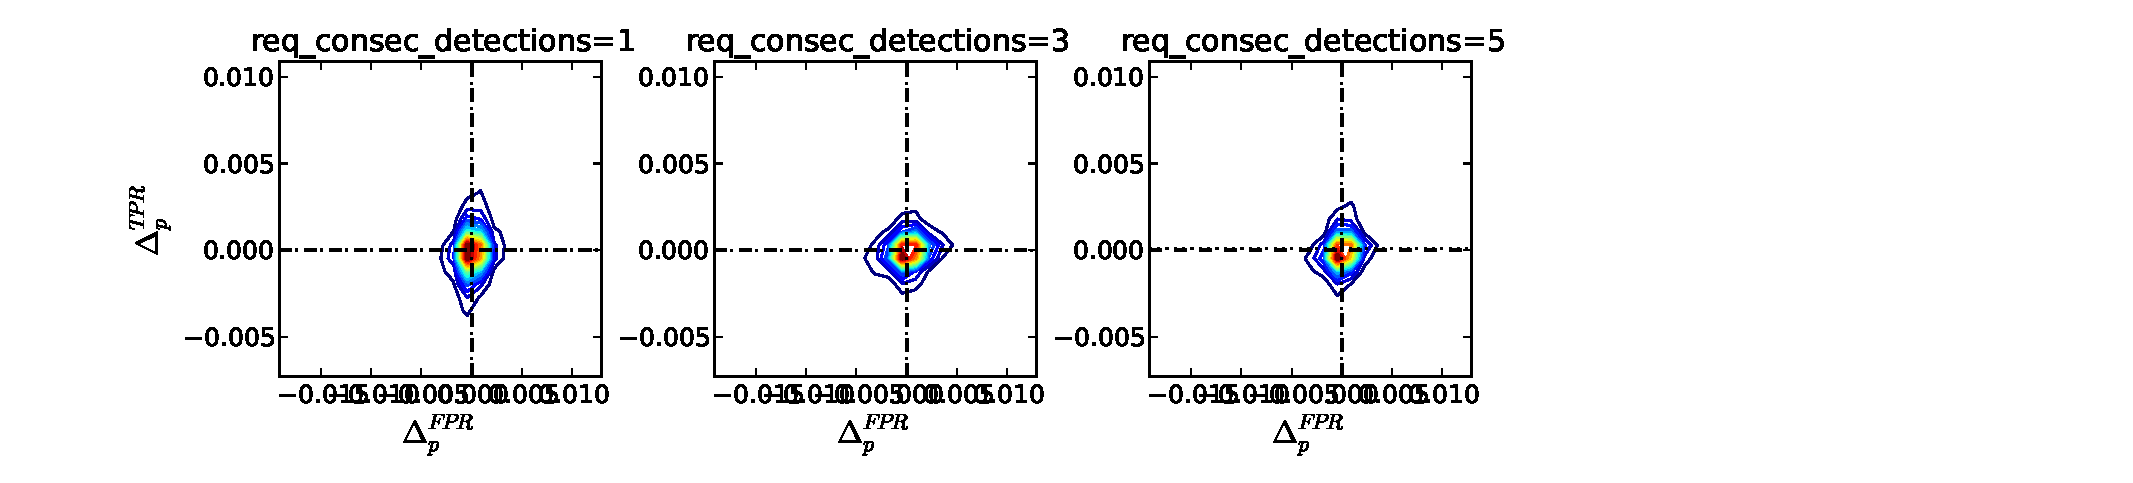
\includegraphics[height=1.5in]{../fig/final/delta_hist_sec/w_smooth/req_consec_detections}
\end{center}
\caption{\label{fig:delta_sec4} Secondary effects of parameters for a varying \vt{WSmooth}}
\end{figure}

\begin{figure}[!h]
\begin{center}
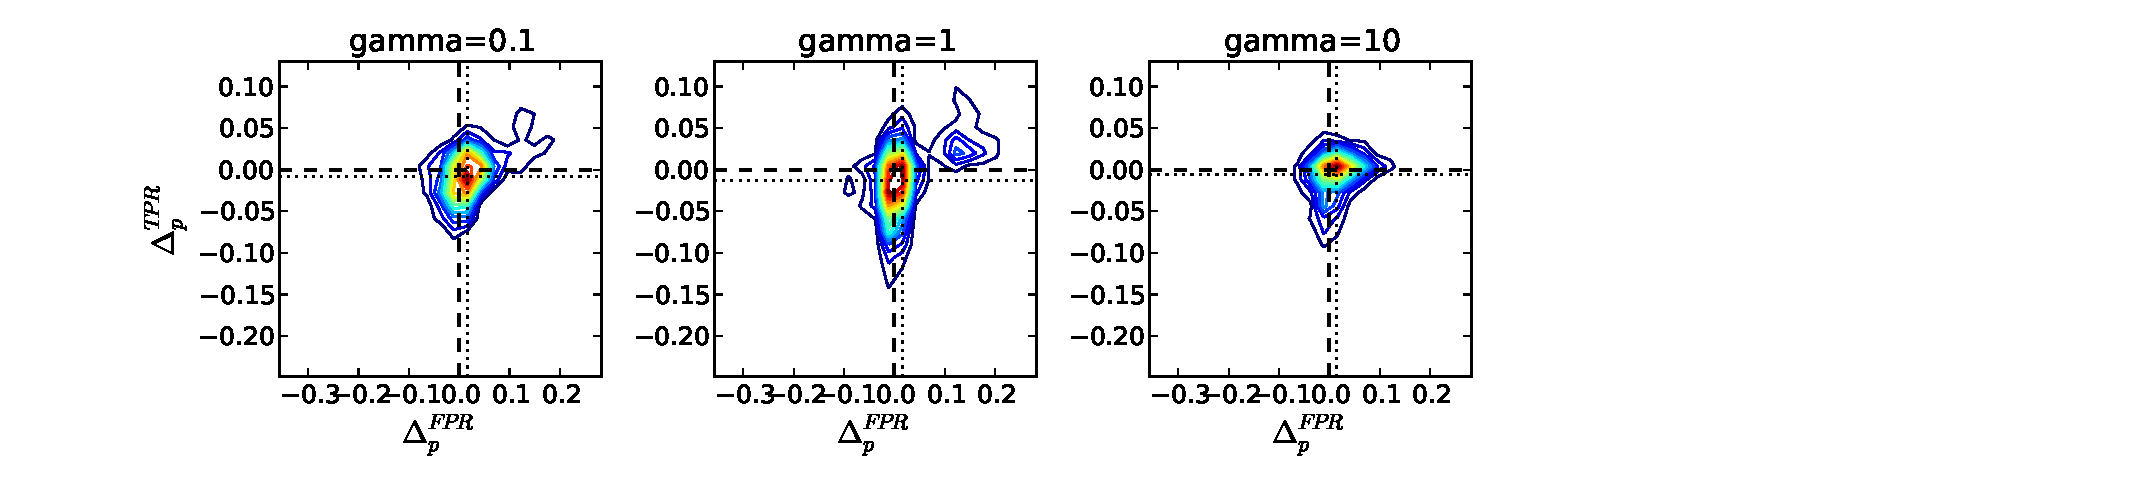
\includegraphics[height=1.5in]{../fig/final/delta_hist_sec/detection_window_hrs/gamma}
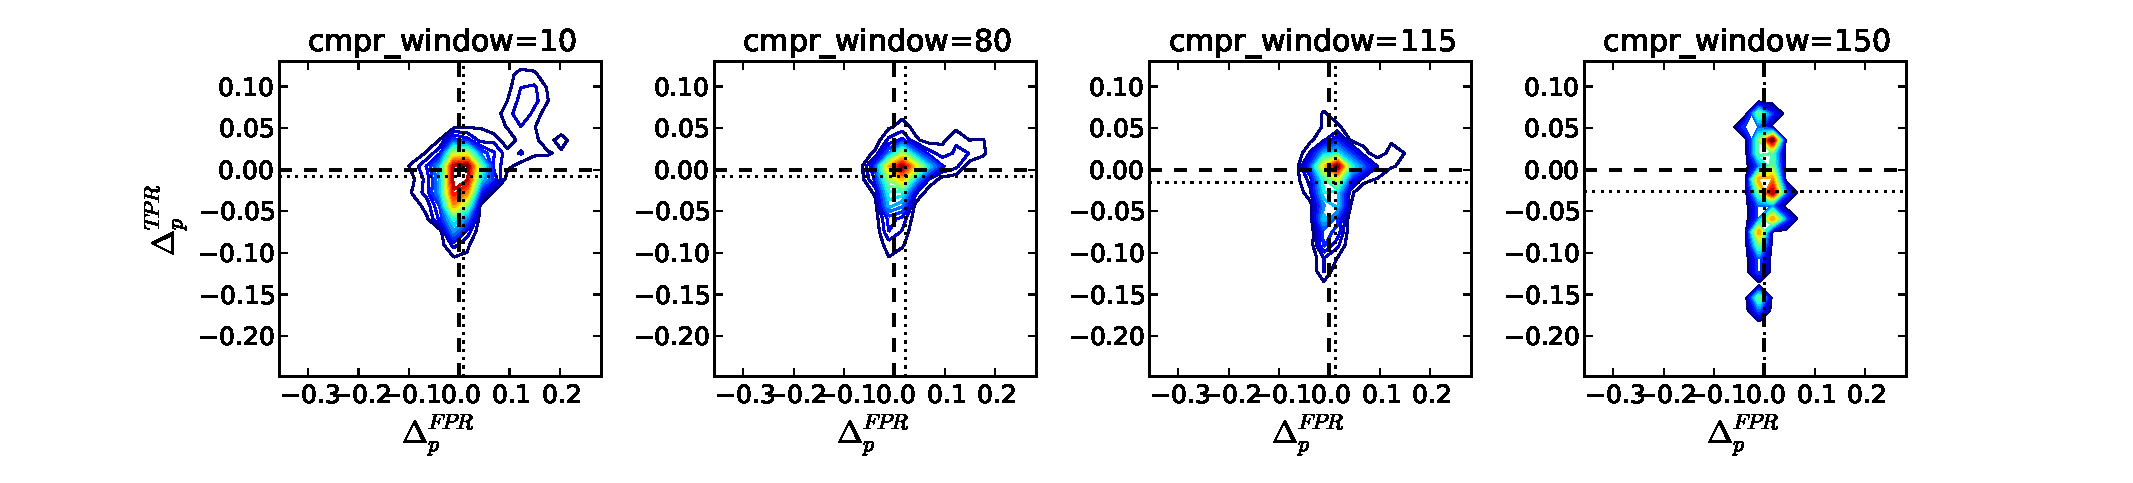
\includegraphics[height=1.5in]{../fig/final/delta_hist_sec/detection_window_hrs/cmpr_window}
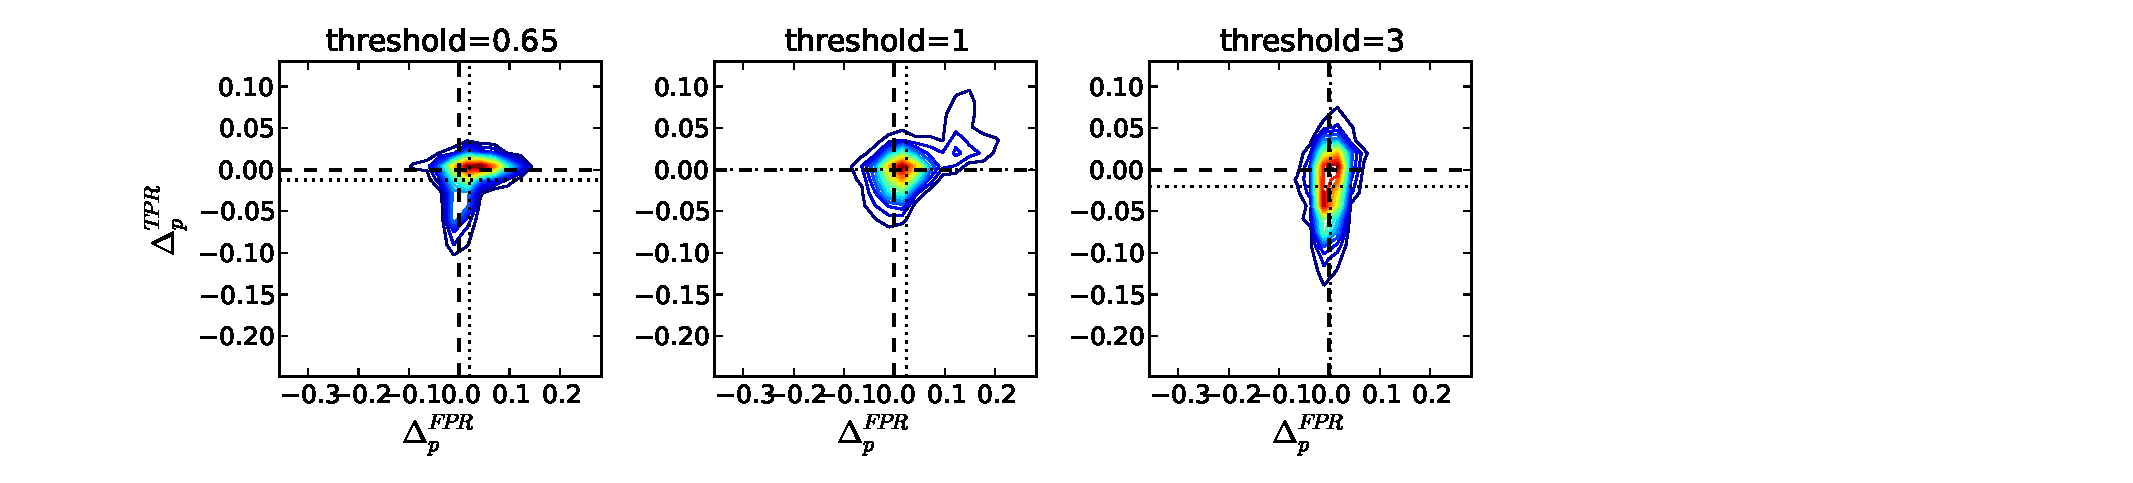
\includegraphics[height=1.5in]{../fig/final/delta_hist_sec/detection_window_hrs/threshold}
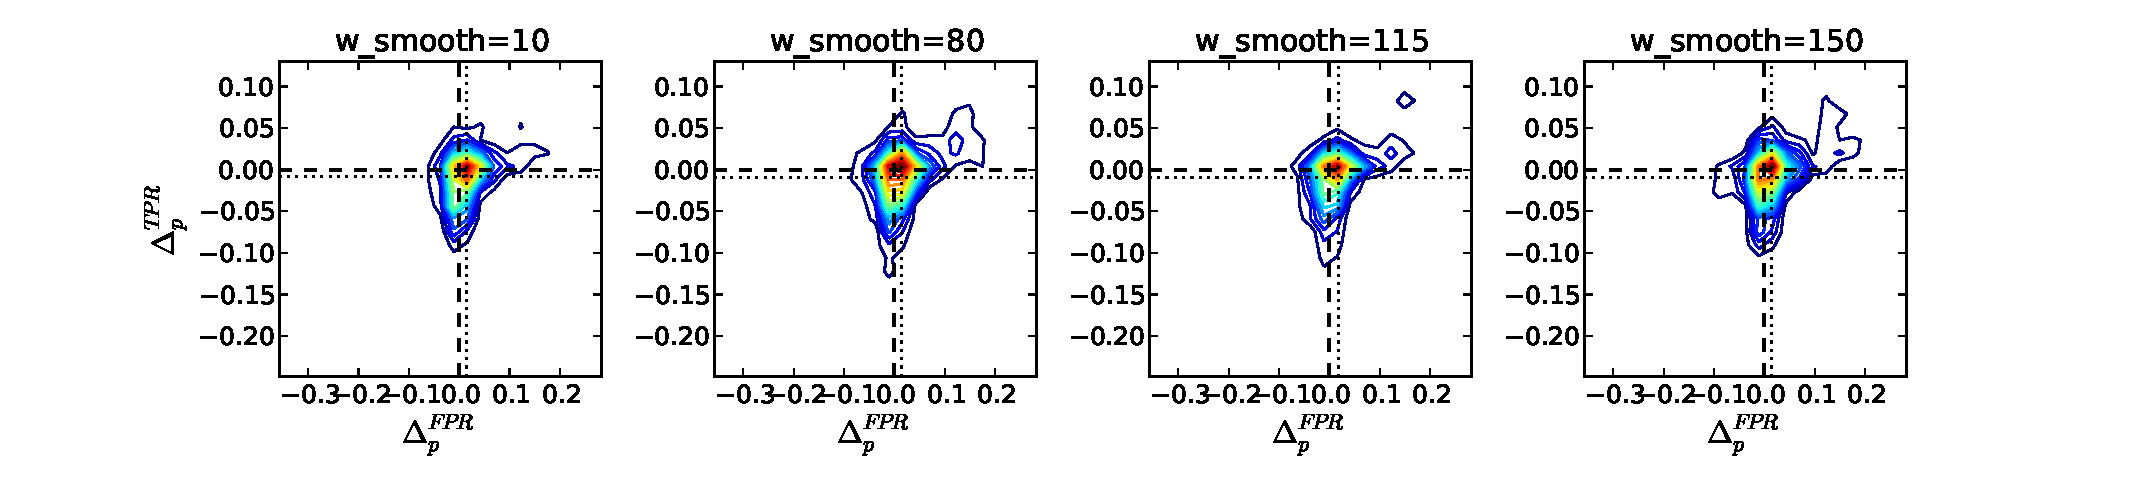
\includegraphics[height=1.5in]{../fig/final/delta_hist_sec/detection_window_hrs/w_smooth}
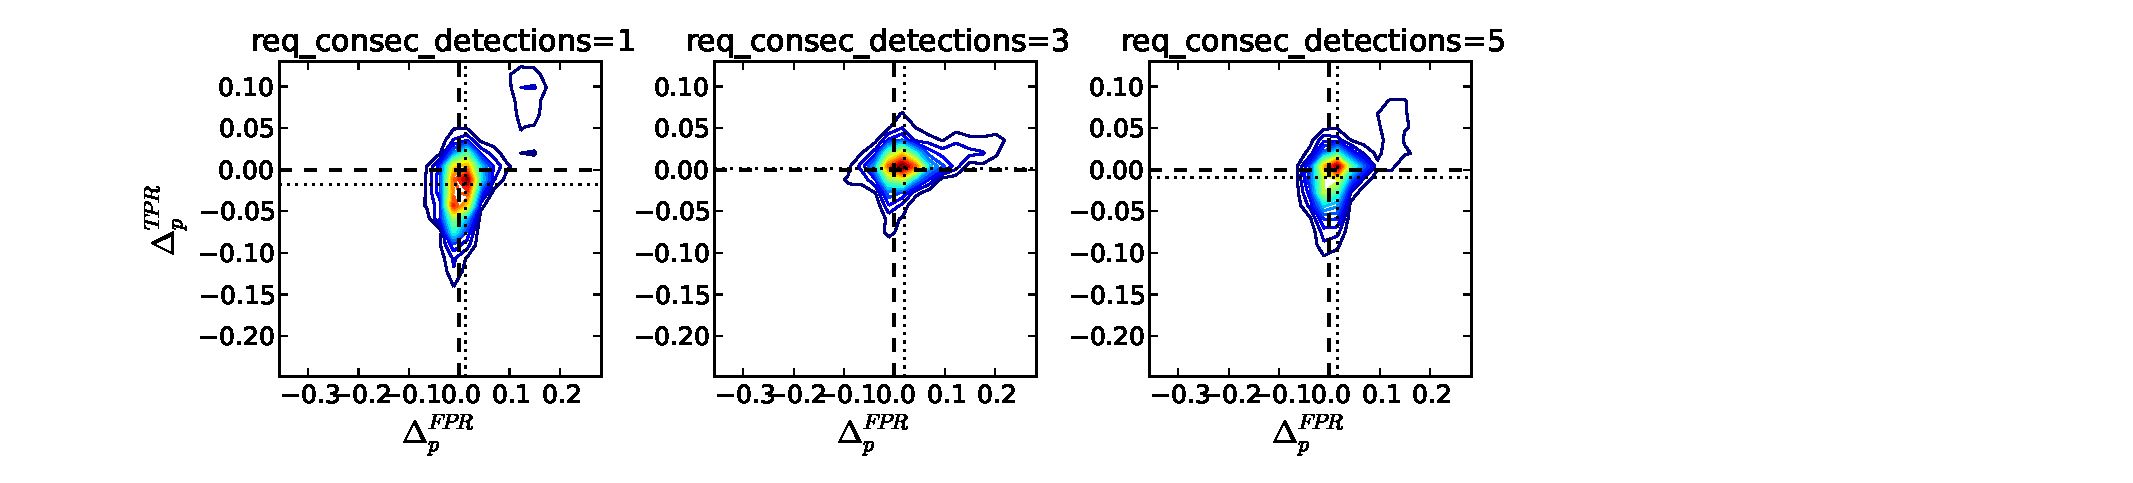
\includegraphics[height=1.5in]{../fig/final/delta_hist_sec/detection_window_hrs/req_consec_detections}
\end{center}
\caption{\label{fig:delta_sec5} Secondary effects of parameters for a varying \vt{DetectionWindowHrs}}
\end{figure}

\begin{figure}[!h]
\begin{center}
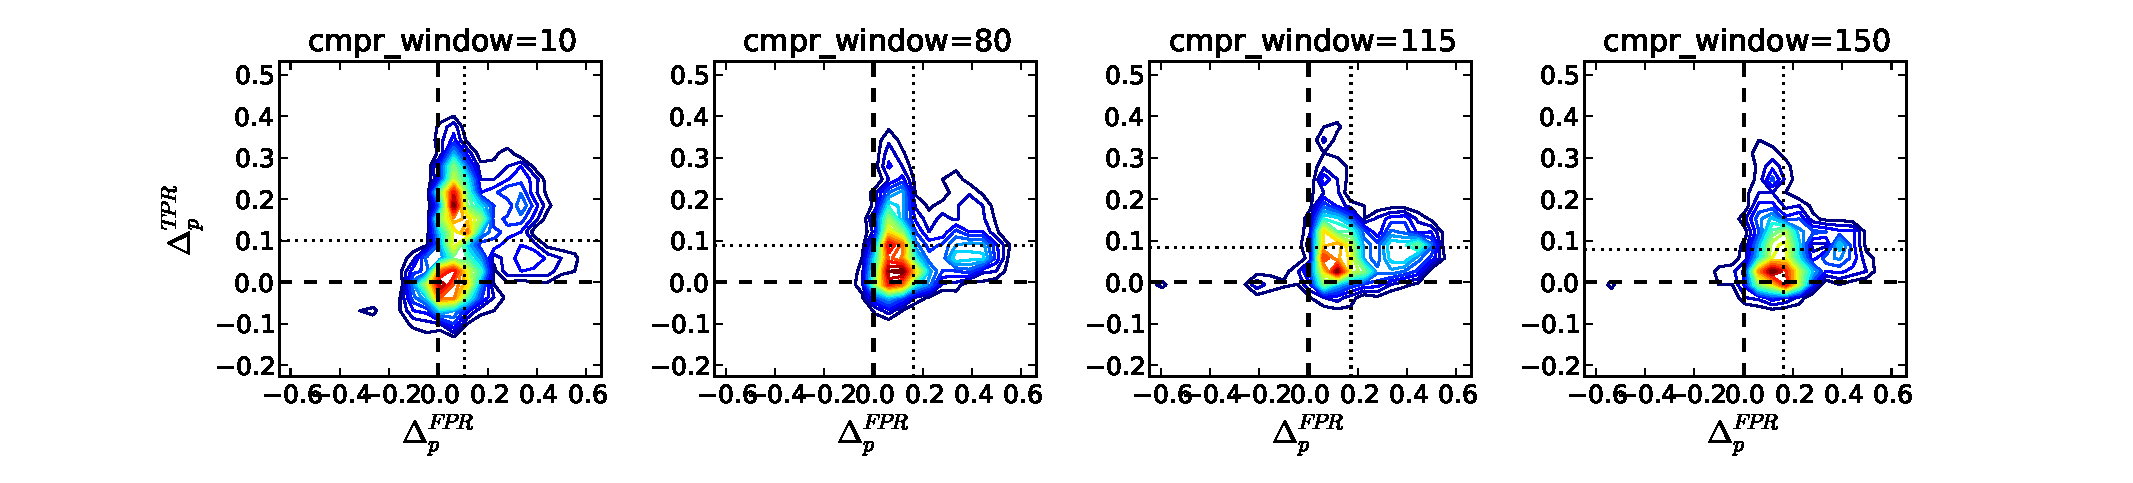
\includegraphics[height=1.5in]{../fig/final/delta_hist_sec/gamma/cmpr_window}
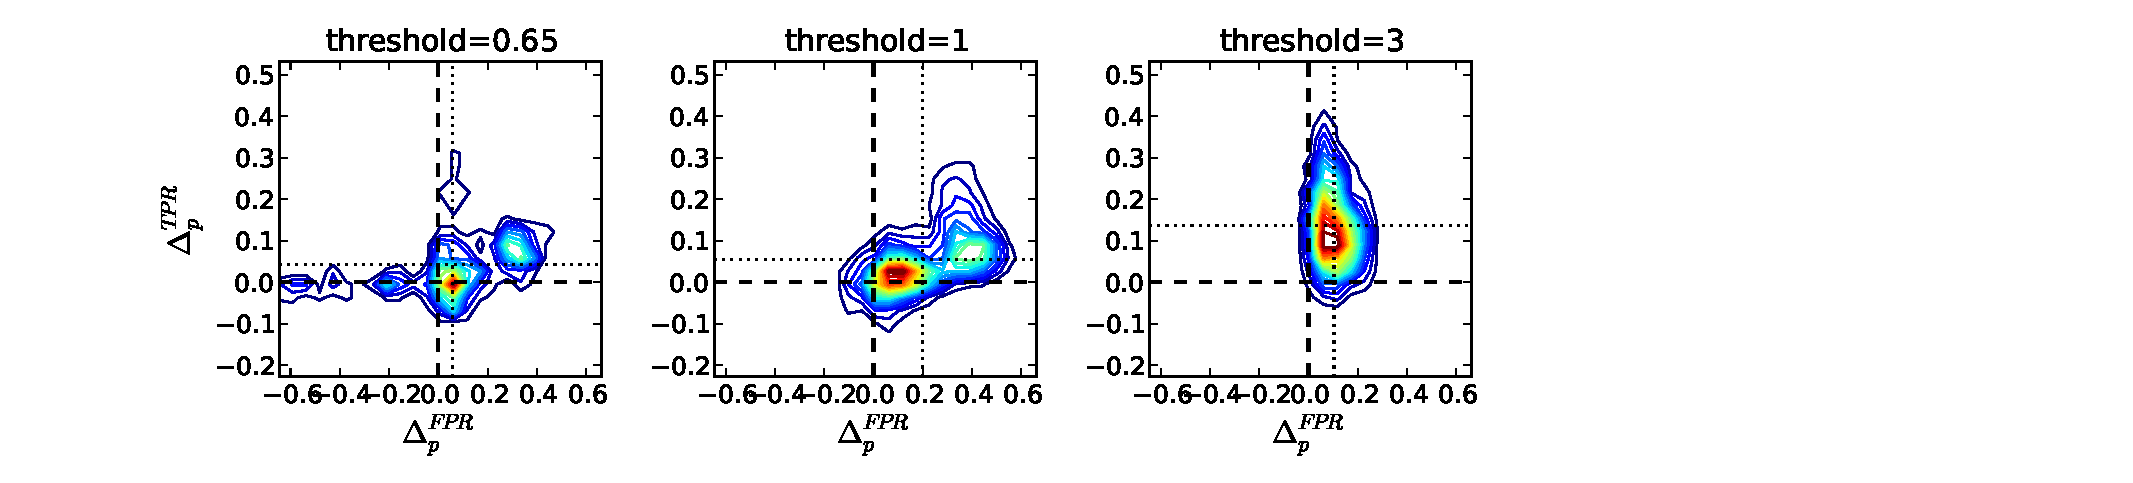
\includegraphics[height=1.5in]{../fig/final/delta_hist_sec/gamma/threshold}
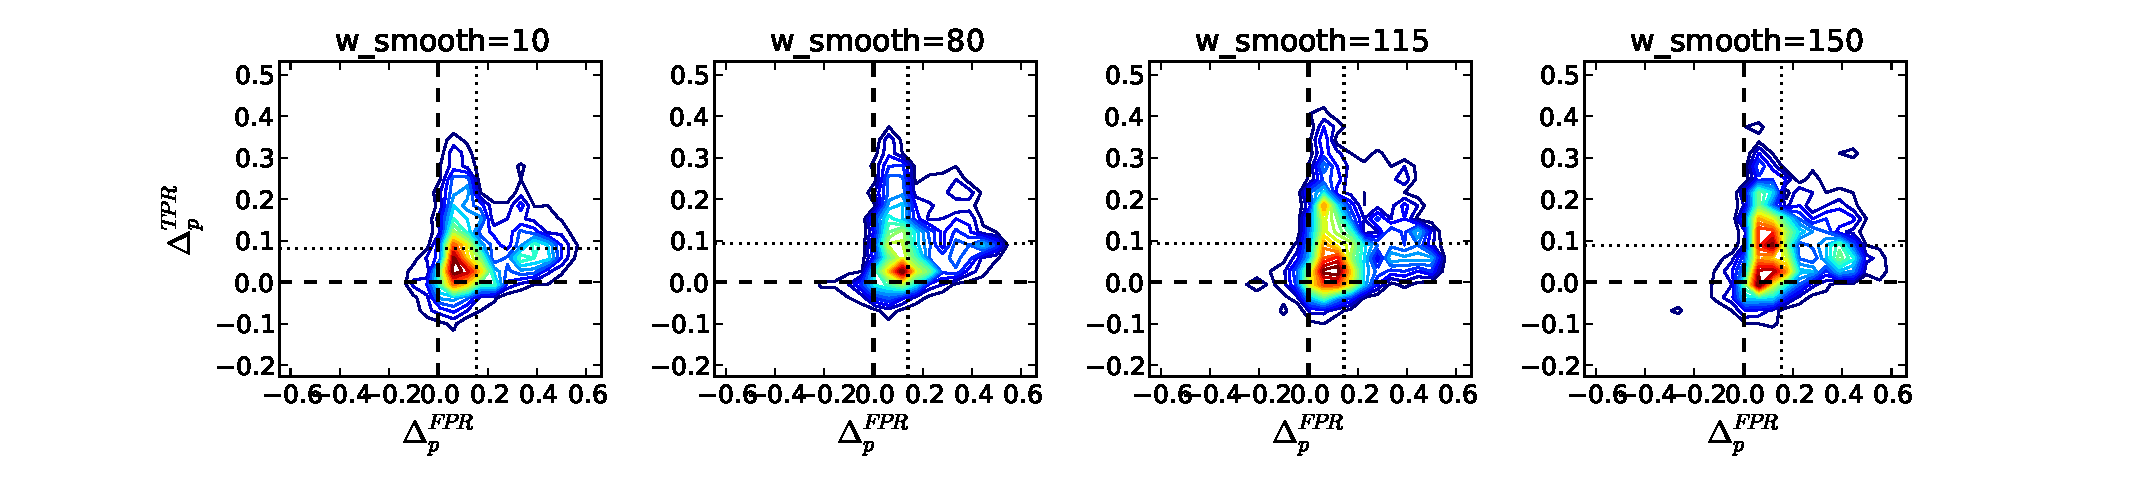
\includegraphics[height=1.5in]{../fig/final/delta_hist_sec/gamma/w_smooth}
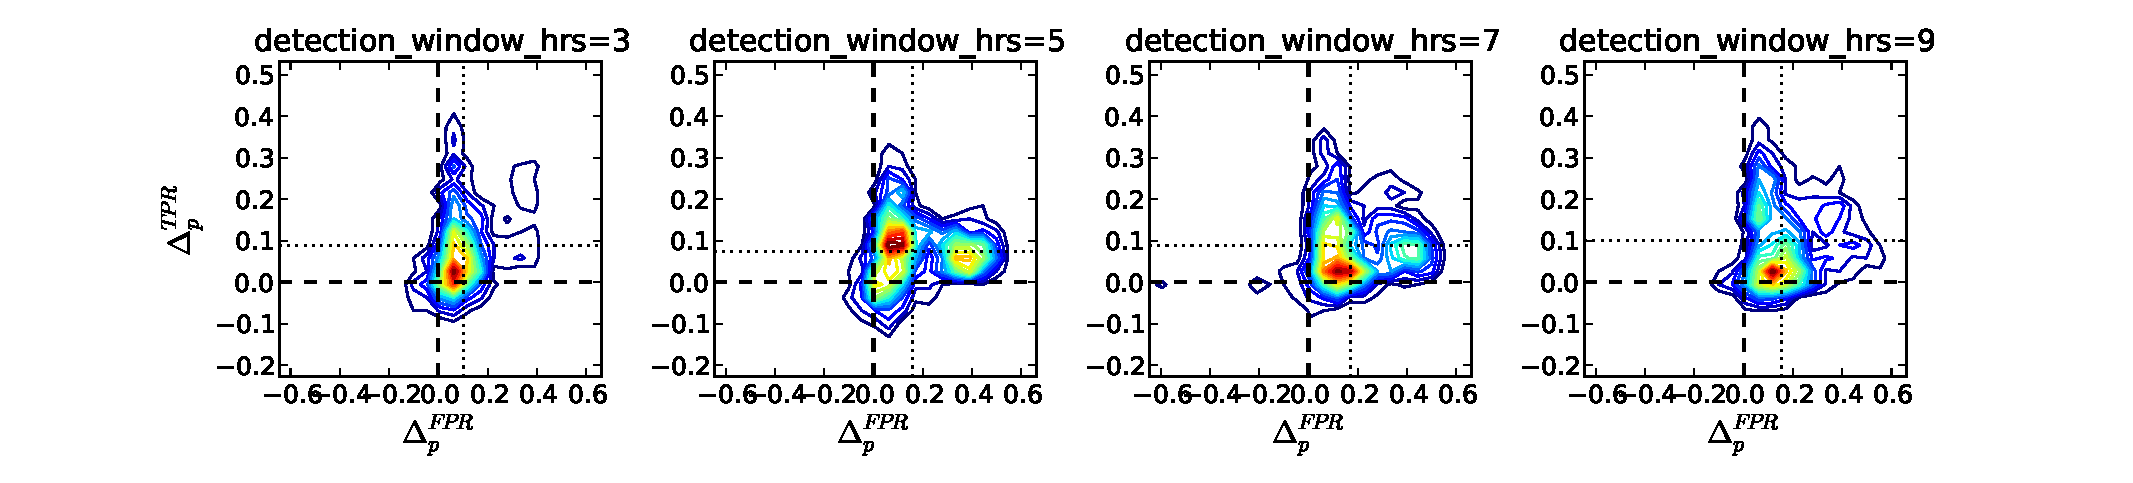
\includegraphics[height=1.5in]{../fig/final/delta_hist_sec/gamma/detection_window_hrs}
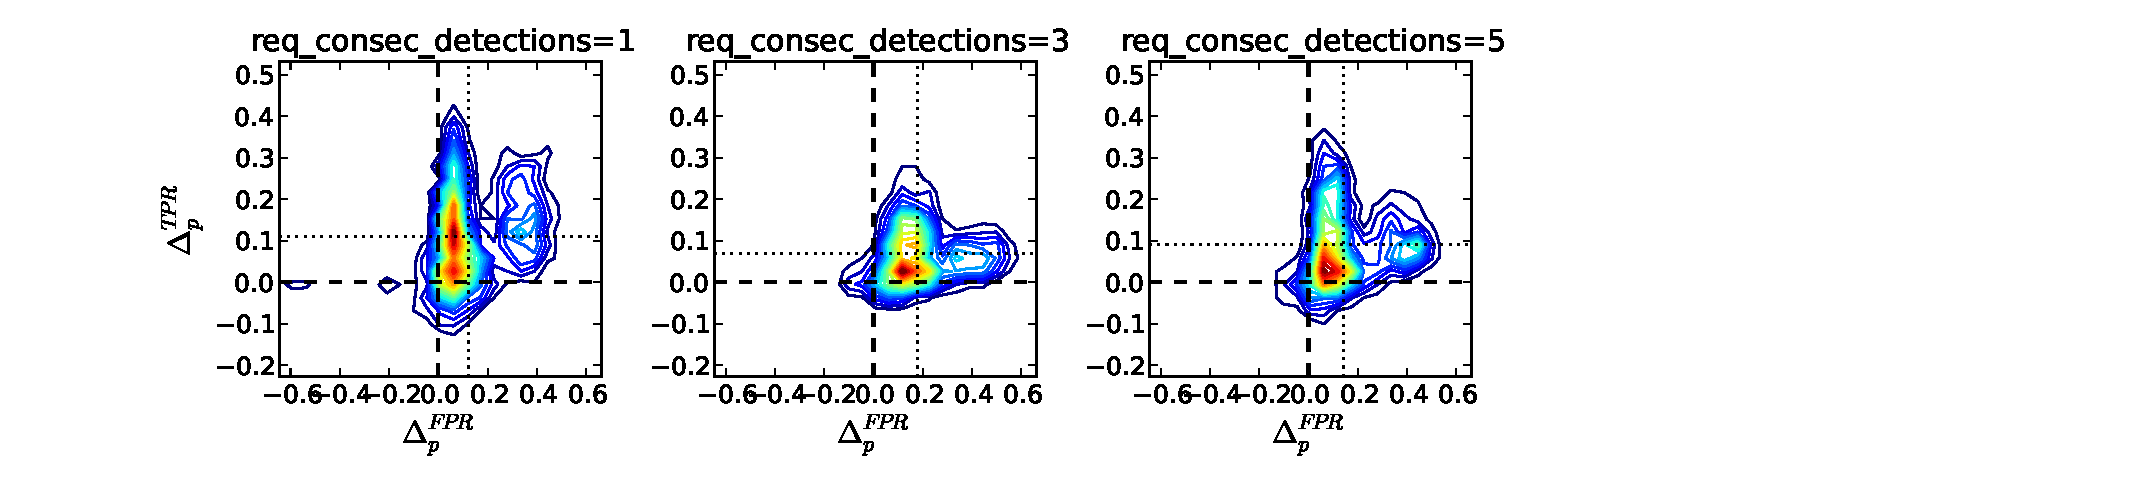
\includegraphics[height=1.5in]{../fig/final/delta_hist_sec/gamma/req_consec_detections}
\end{center}
\caption{\label{fig:delta_sec6} Secondary effects of parameters for a varying \vt{ReqConsecDetections}}
\end{figure}

\clearpage
% Top and bottom ROC curves
Figures \ref{fig:delta_top_bottom1f,fig:delta_top_bottom1t,fig:delta_top_bottom2f,fig:delta_top_bottom2t,fig:delta_top_bottom3f,fig:delta_top_bottom3t,fig:delta_top_bottom4f,fig:delta_top_bottom4t,fig:delta_top_bottom5f,fig:delta_top_bottom5t,fig:delta_top_bottom6f,fig:delta_top_bottom6t} show the top and bottom ROC curves ranked by mean $\Delta_p^{FPR}$ and mean $\Delta_p^{TPR}$. For each varying parameter, the ROC curves with the top mean $\Delta_p^{FPR}$ show the values of the constant parameters for which the variable parameter has the largest positive effect on $FPR$. Similarly, the bottom-ranked ROC curves represent ROC curves for which the variable parameter has the lowest positive (possibly negative) effect on $FPR$.

\begin{figure}[!h]
\begin{center}
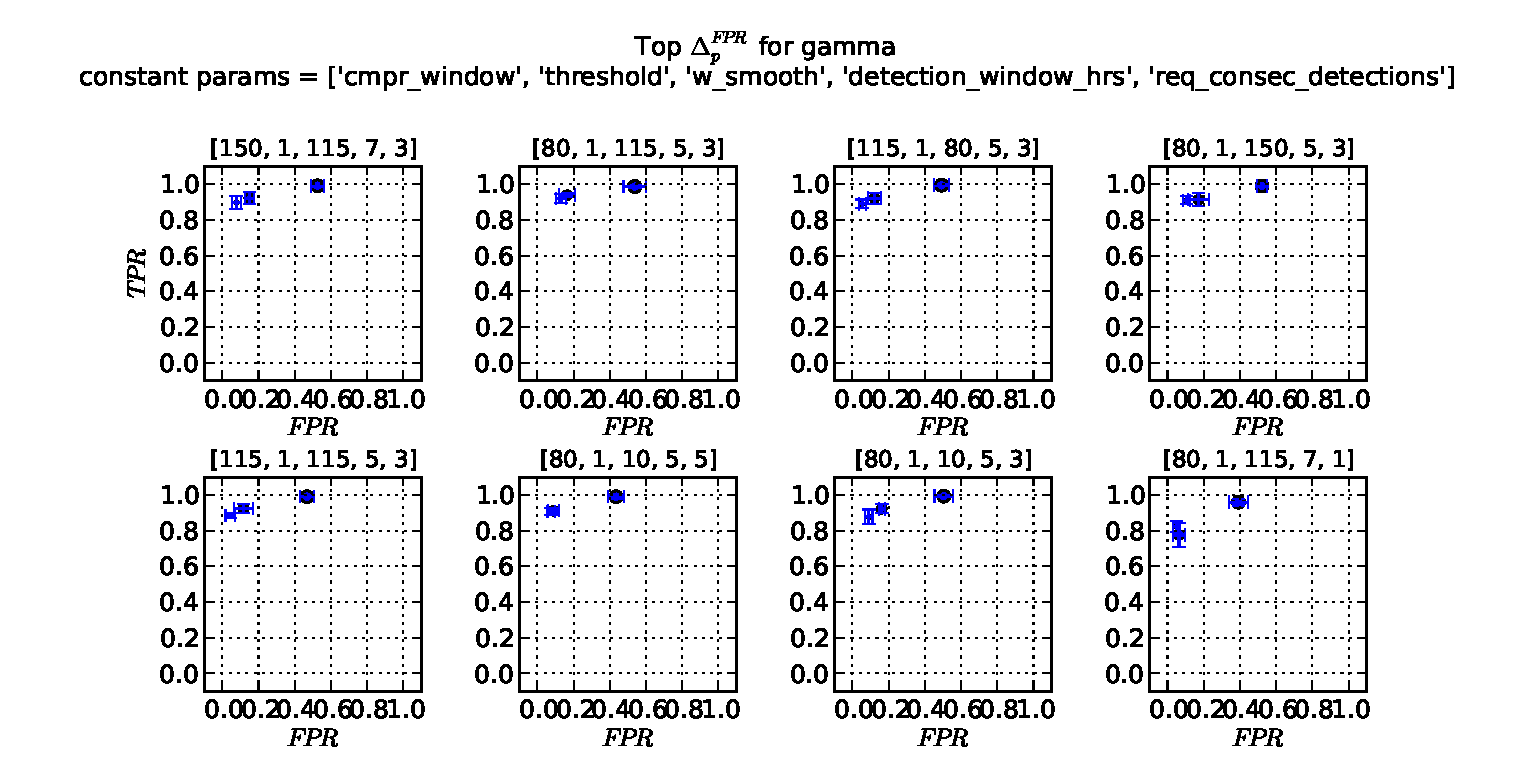
\includegraphics[height=3in]{../fig/final/top_fpr/gamma}
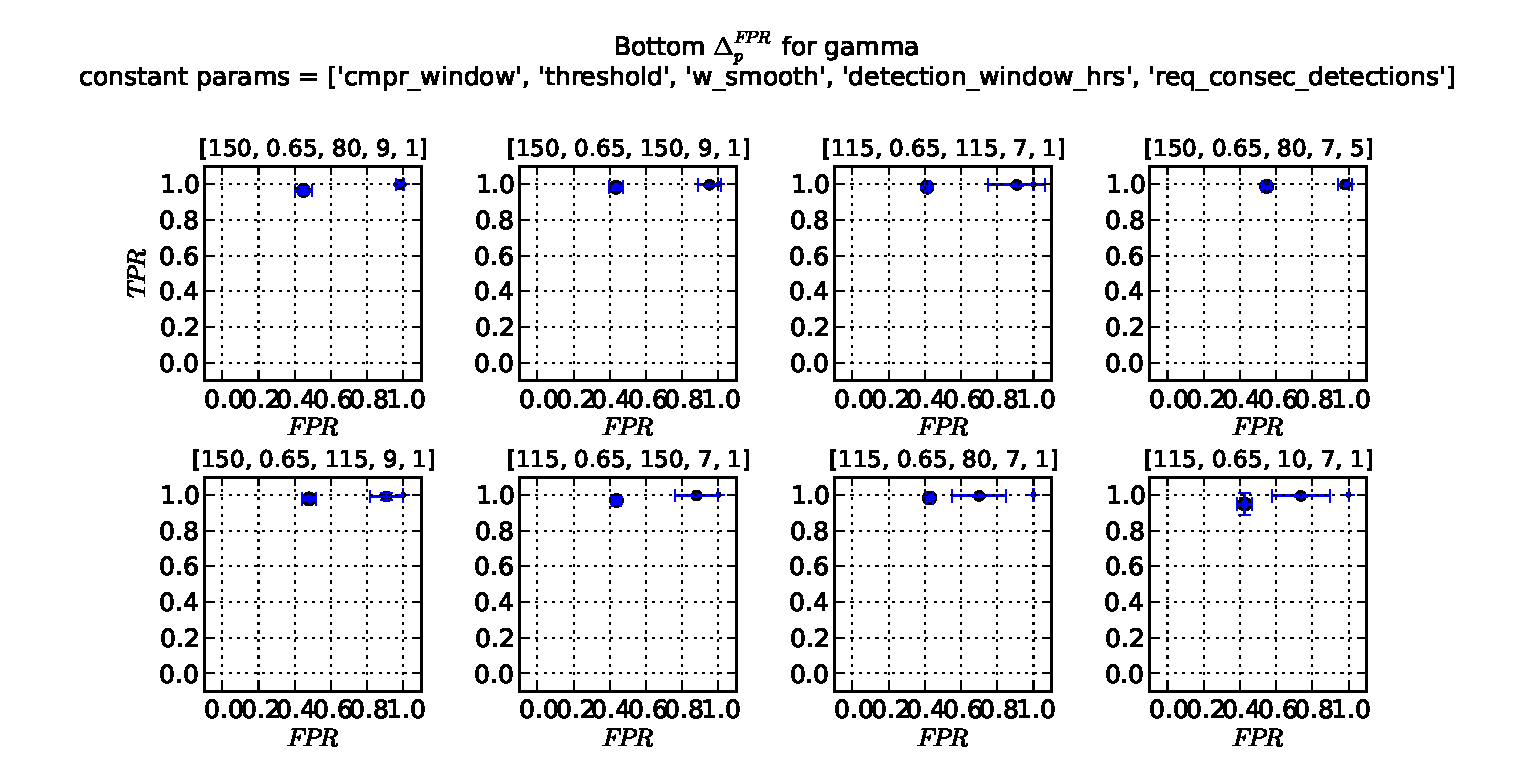
\includegraphics[height=3in]{../fig/final/bottom_fpr/gamma}
\end{center}
\caption{\label{fig:delta_top_bottom1f} Top and bottom $\Delta_p^{FPR}$ for \vt{Gamma}}
\end{figure}


\begin{figure}[!h]
\begin{center}
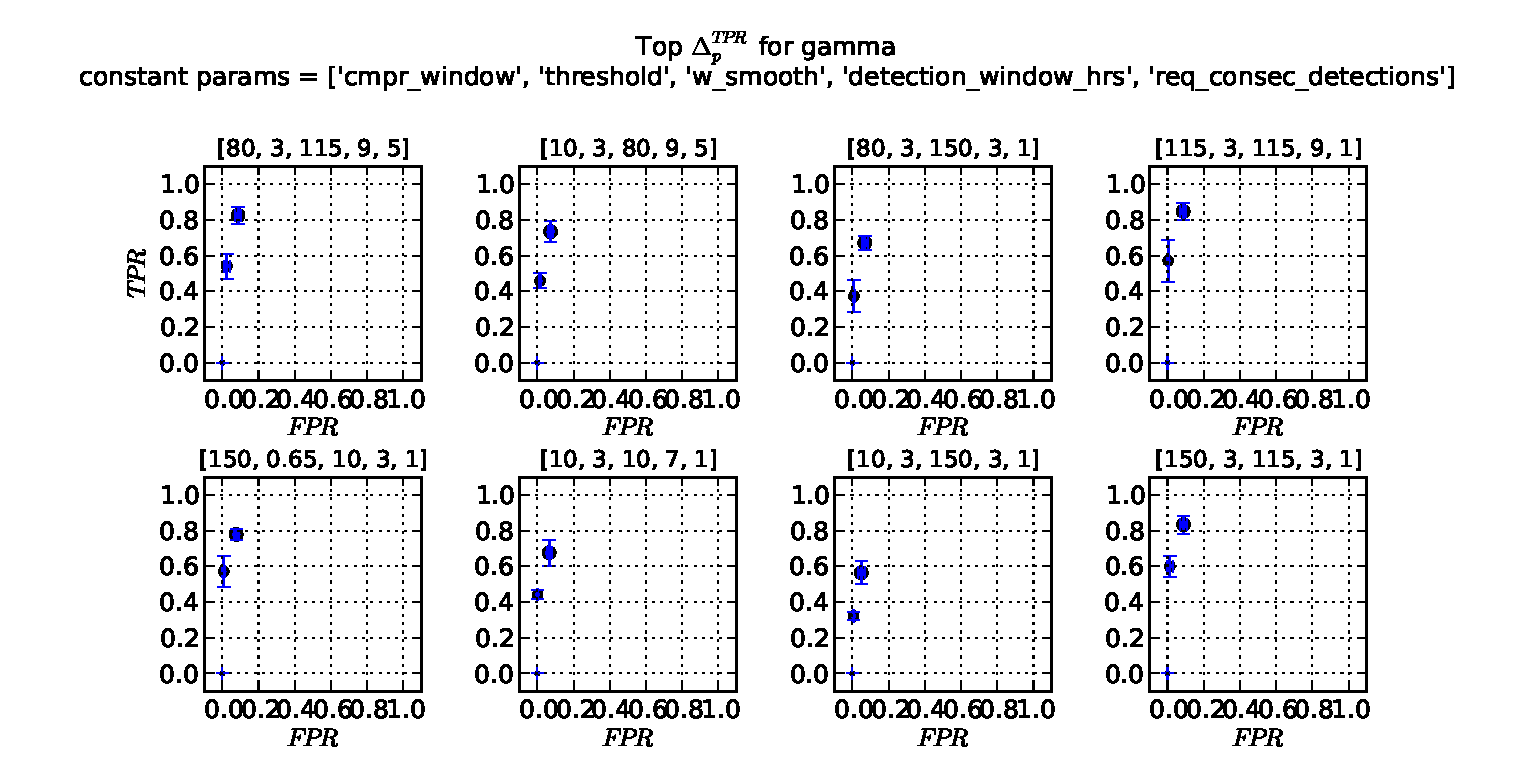
\includegraphics[height=3in]{../fig/final/top_tpr/gamma}
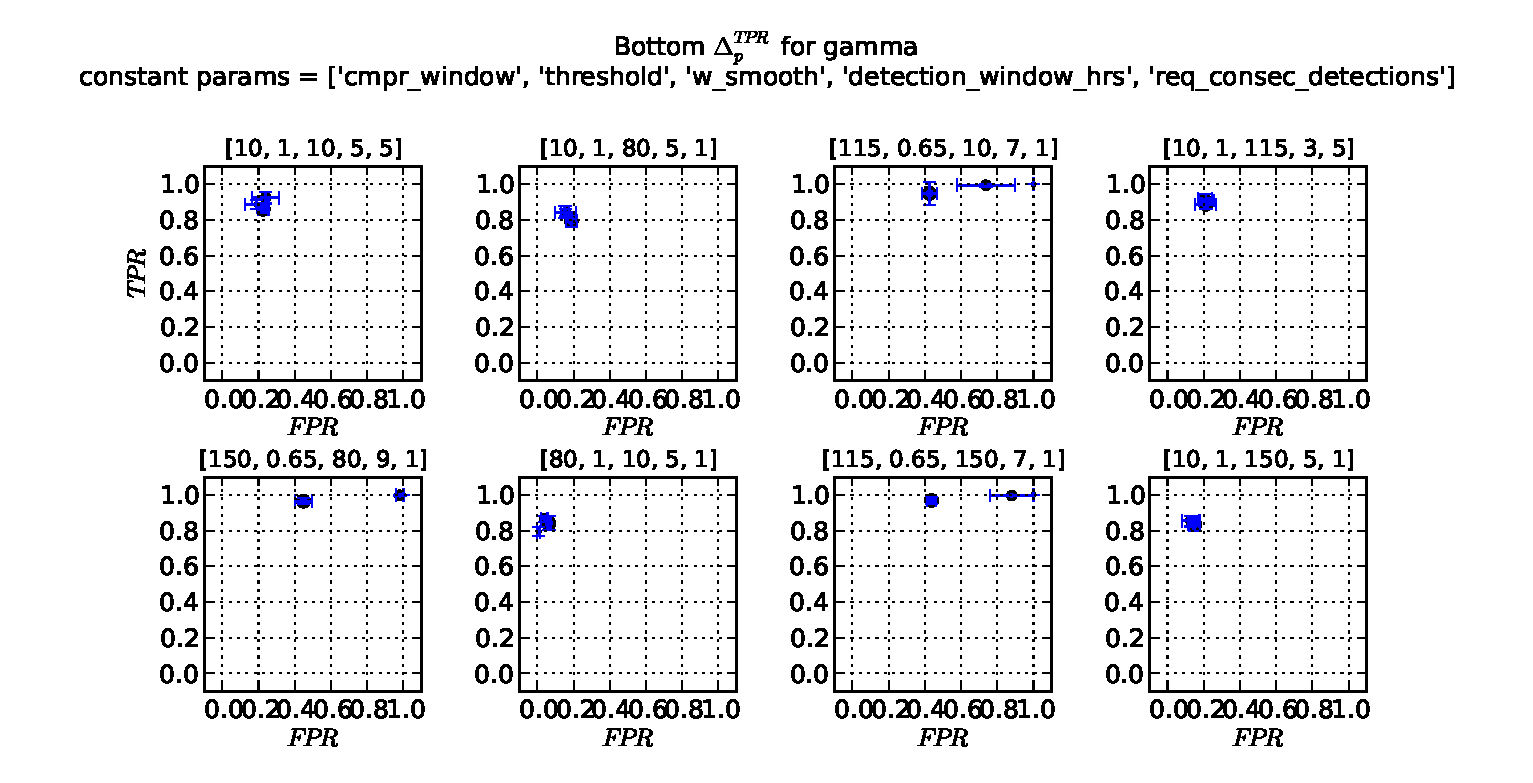
\includegraphics[height=3in]{../fig/final/bottom_tpr/gamma}
\end{center}
\caption{\label{fig:delta_top_bottom1t} Top and bottom $\Delta_p^{TPR}$ for \vt{Gamma}}
\end{figure}




\begin{figure}[!h]
\begin{center}
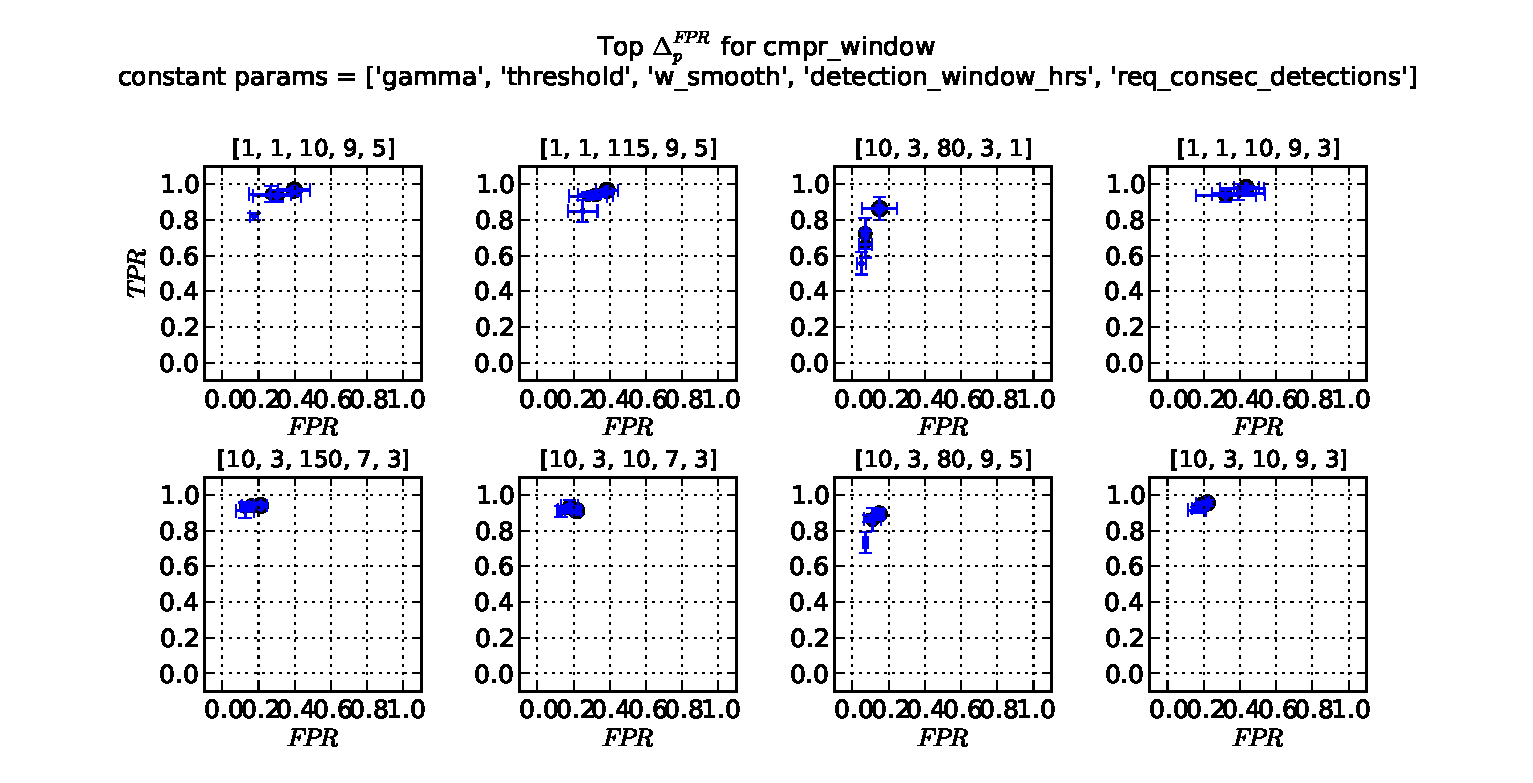
\includegraphics[height=3in]{../fig/final/top_fpr/cmpr_window}
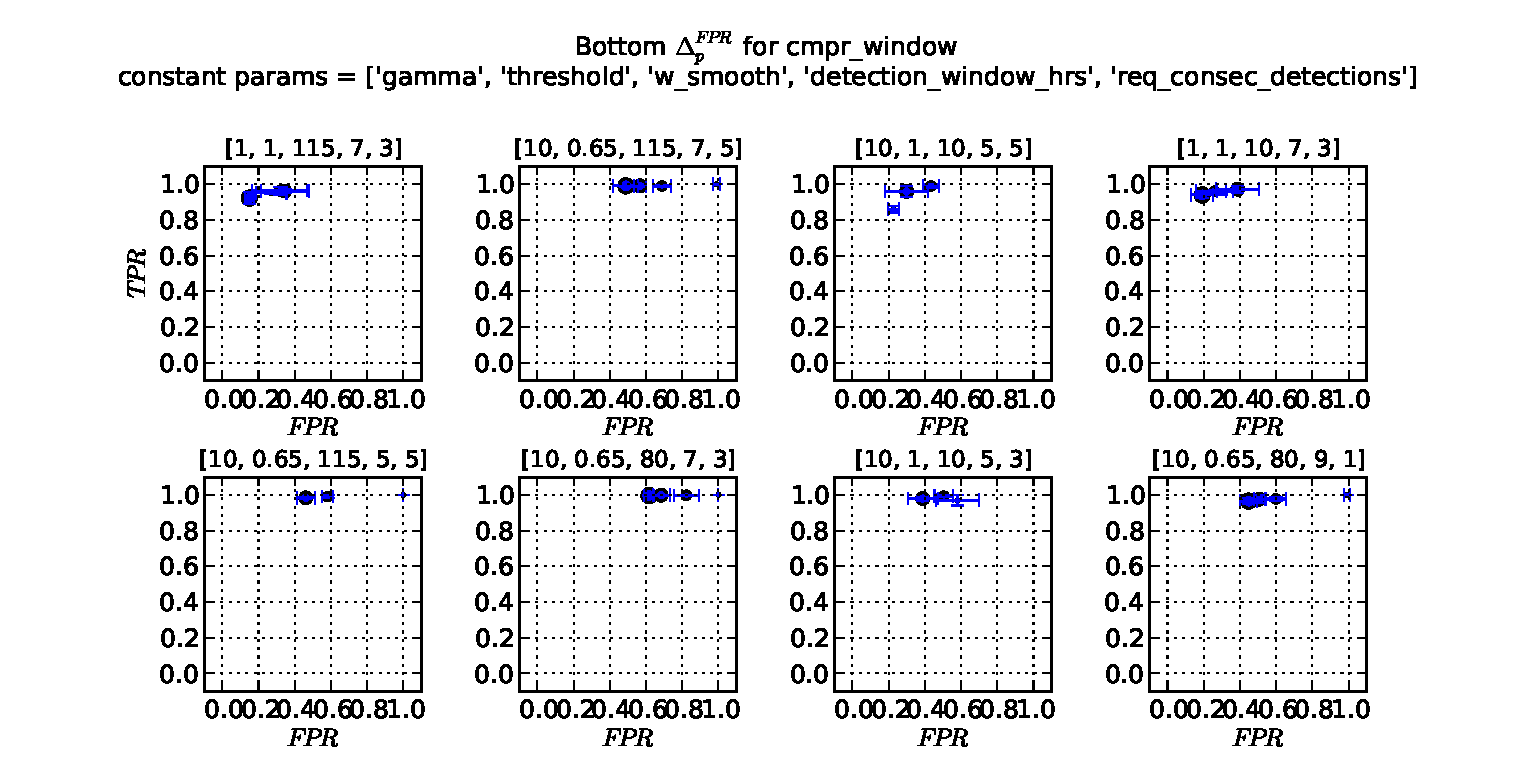
\includegraphics[height=3in]{../fig/final/bottom_fpr/cmpr_window}
\end{center}
\caption{\label{fig:delta_top_bottom2f} Top and bottom $\Delta_p^{FPR}$ for \vt{CmprWindow}}
\end{figure}

\begin{figure}[!h]
\begin{center}
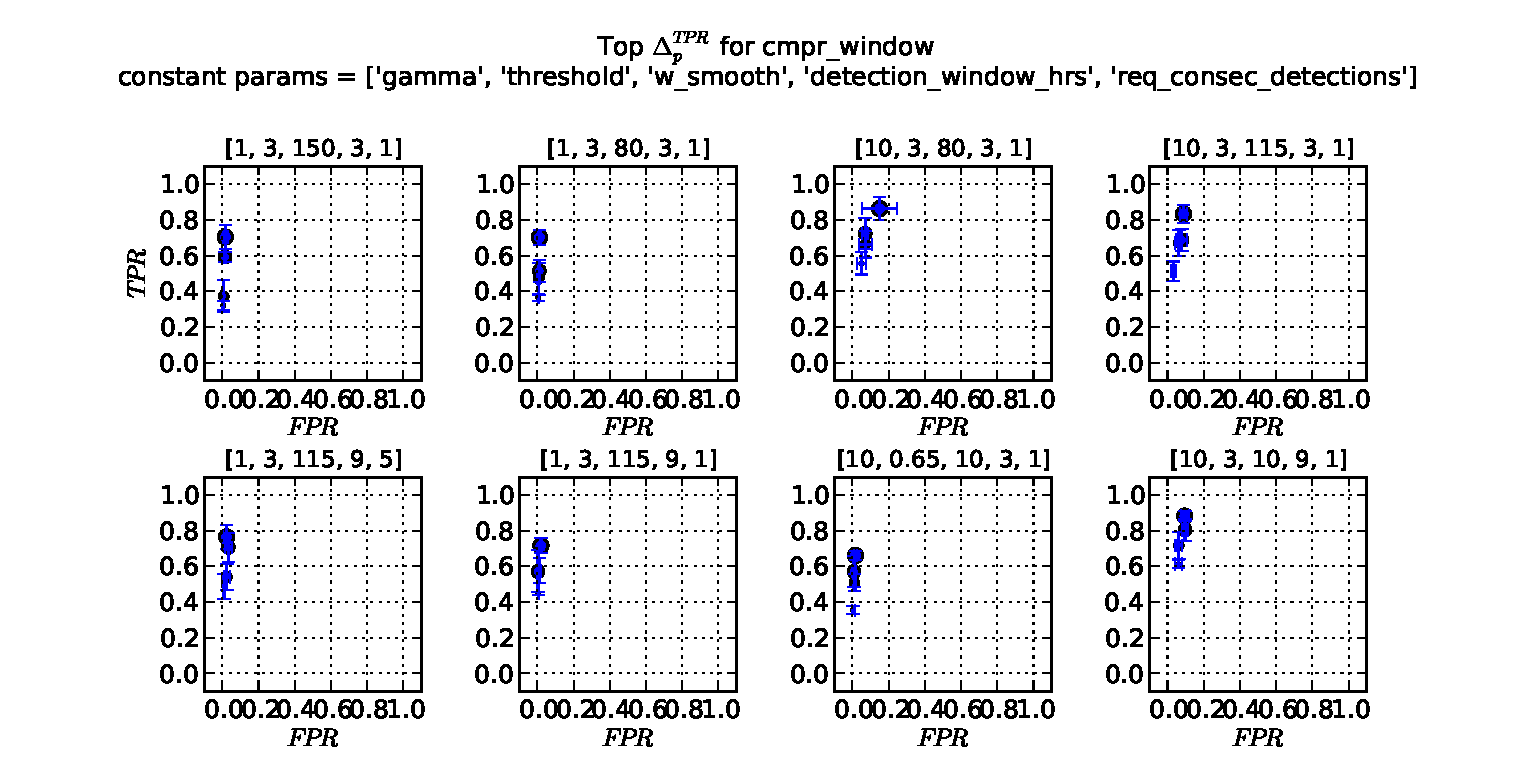
\includegraphics[height=3in]{../fig/final/top_tpr/cmpr_window}
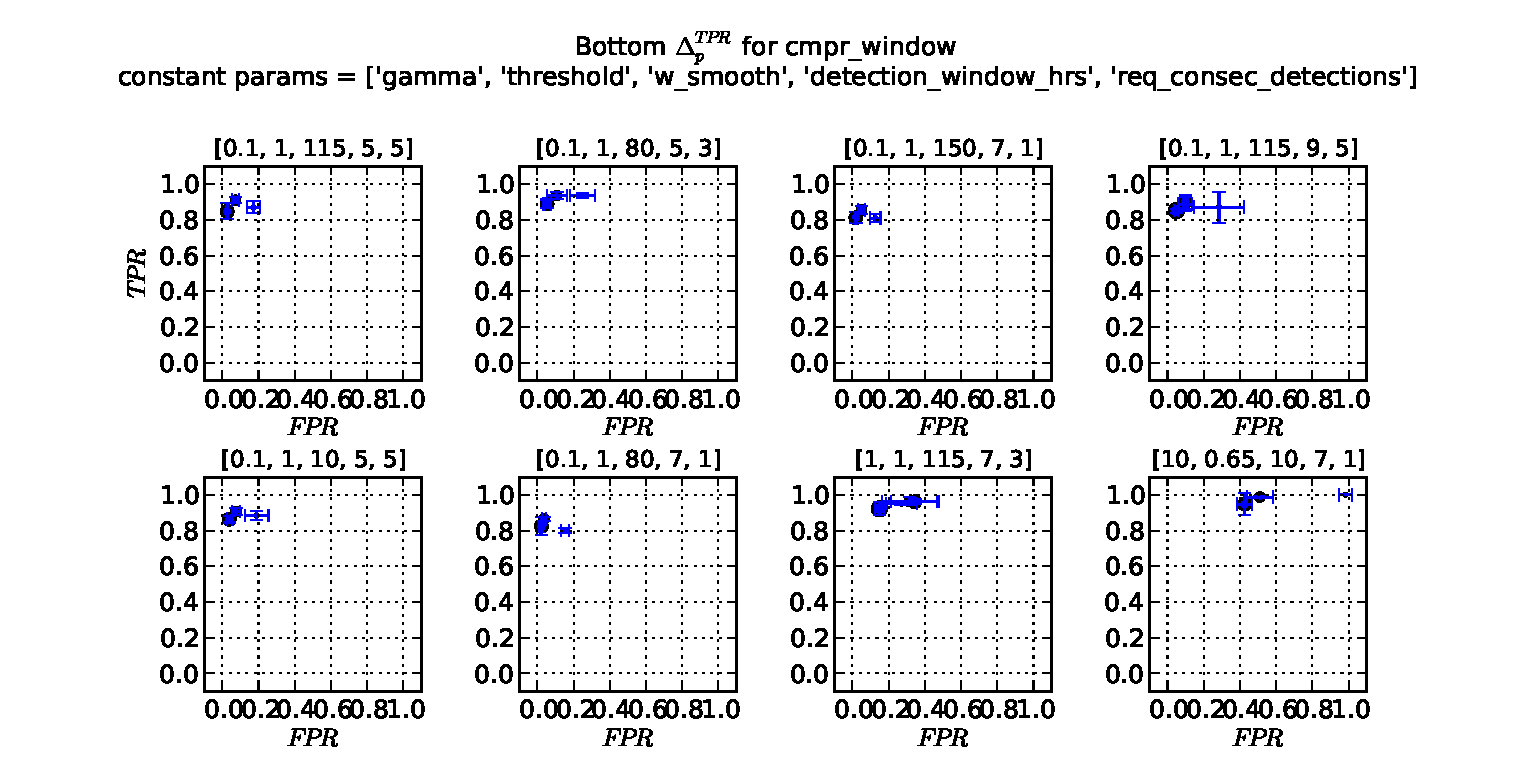
\includegraphics[height=3in]{../fig/final/bottom_tpr/cmpr_window}
\end{center}
\caption{\label{fig:delta_top_bottom2t} Top and bottom $\Delta_p^{TPR}$ for \vt{CmprWindow}}
\end{figure}



% Threshold
\begin{figure}[!h]
\begin{center}
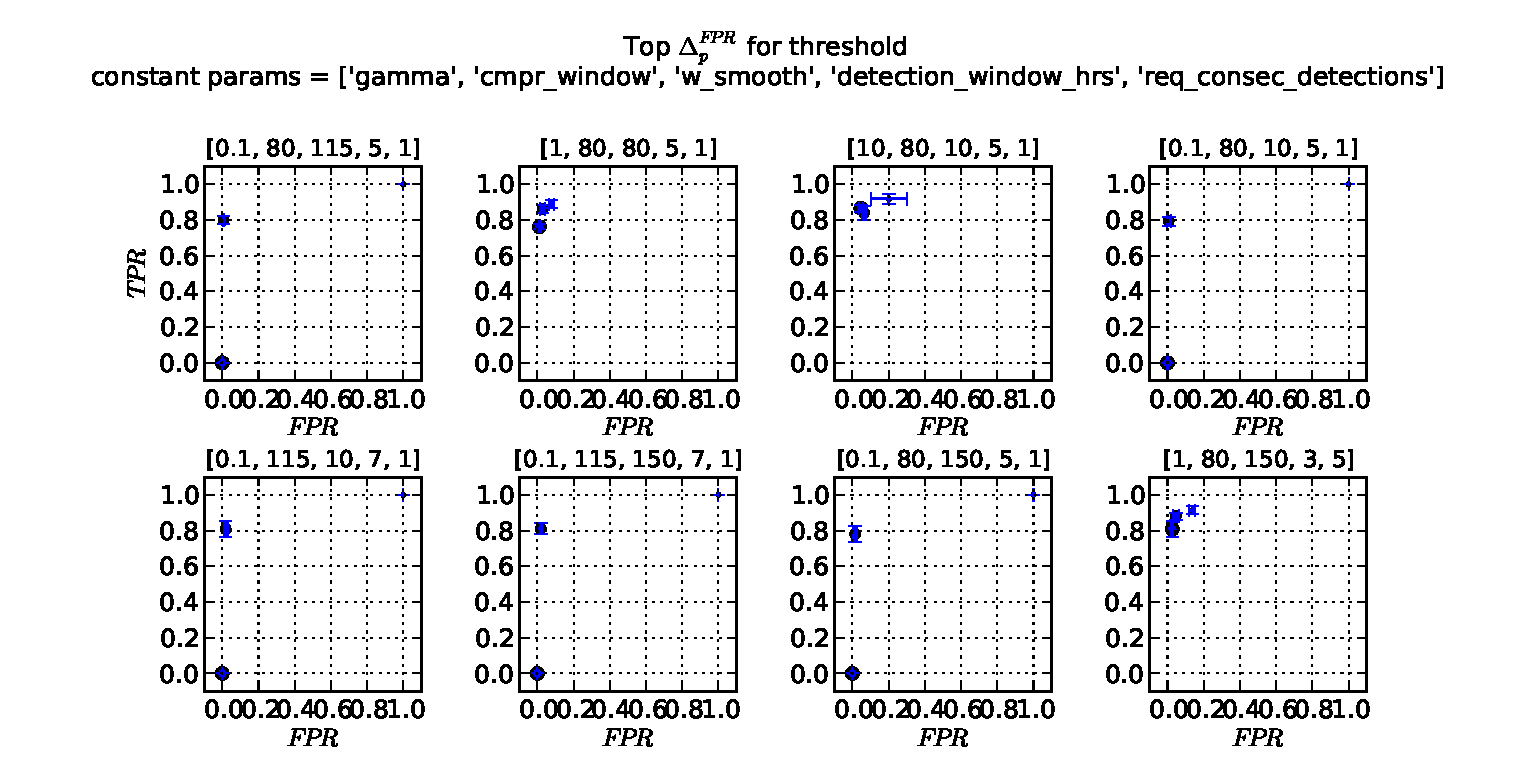
\includegraphics[height=3in]{../fig/final/top_fpr/threshold}
\includegraphics[height=3in]{../fig/final/bottom_fpr/threshold}
\end{center}
\caption{\label{fig:delta_top_bottom3f} Top and bottom $\Delta_p^{FPR}$ for \vt{Threshold}}
\end{figure}


\begin{figure}[!h]
\begin{center}
\includegraphics[height=3in]{../fig/final/top_tpr/threshold}
\includegraphics[height=3in]{../fig/final/bottom_tpr/threshold}
\end{center}
\caption{\label{fig:delta_top_bottom3t} Top and bottom $\Delta_p^{TPR}$ for \vt{Threshold}}
\end{figure}



% WSmooth
\begin{figure}[!h]
\begin{center}
\includegraphics[height=3in]{../fig/final/top_fpr/w_smooth}
\includegraphics[height=3in]{../fig/final/bottom_fpr/w_smooth}
\end{center}
\caption{\label{fig:delta_top_bottom4f} Top and bottom $\Delta_p^{FPR}$ for \vt{WSmooth}}
\end{figure}

\begin{figure}[!h]
\begin{center}
\includegraphics[height=3in]{../fig/final/top_tpr/w_smooth}
\includegraphics[height=3in]{../fig/final/bottom_tpr/w_smooth}
\end{center}
\caption{\label{fig:delta_top_bottom4t} Top and bottom $\Delta_p^{TPR}$ for \vt{WSmooth}}
\end{figure}


% DetectionWindowHrs
\begin{figure}[!h]
\begin{center}
\includegraphics[height=3in]{../fig/final/top_fpr/detection_window_hrs}
\includegraphics[height=3in]{../fig/final/bottom_fpr/detection_window_hrs}
\end{center}
\caption{\label{fig:delta_top_bottom5f} Top and bottom $\Delta_p^{FPR}$ for \vt{DetectionWindowHrs}}
\end{figure}

\begin{figure}[!h]
\begin{center}
\includegraphics[height=3in]{../fig/final/top_tpr/detection_window_hrs}
\includegraphics[height=3in]{../fig/final/bottom_tpr/detection_window_hrs}
\end{center}
\caption{\label{fig:delta_top_bottom5t} Top and bottom $\Delta_p^{TPR}$ for \vt{DetectionWindowHrs}}
\end{figure}

% ReqConsecDetections
\begin{figure}[!h]
\begin{center}
\includegraphics[height=3in]{../fig/final/top_fpr/req_consec_detections}
\includegraphics[height=3in]{../fig/final/bottom_fpr/req_consec_detections}
\end{center}
\caption{\label{fig:delta_top_bottom6f} Top and bottom $\Delta_p^{FPR}$ for \vt{ReqConsecDetections}}
\end{figure}

\begin{figure}[!h]
\begin{center}
\includegraphics[height=3in]{../fig/final/top_tpr/req_consec_detections}
\includegraphics[height=3in]{../fig/final/bottom_tpr/req_consec_detections}
\end{center}
\caption{\label{fig:delta_top_bottom6t} Top and bottom $\Delta_p^{TPR}$ for \vt{ReqConsecDetections}}
\end{figure}

% TODO: Discuss effect on relative detection time

%TODO: Ranking of all combinations of fixed parameters based on tpr (and based
%on fpr). Show many (ranked) thumbnail ROC curves for each varying parameter.

%TODO: Ranking of all combinations of fixed parameters based on pct(deltas >
%0). Restrict to the important params and show delta histograms again, showing a
%consistent up or down movement along the curve. Show many (ranked) thumbnail
%ROC curves for each varying parameter.

% Wait a minute... if varying a parameter moves TPR up and FPR down, isn't
% that... really really good?
\section{Recommendations}
